\documentclass{beamer}
%\documentclass[handout]{beamer}
% packages
\usepackage[utf8]{inputenc}
\usepackage{graphicx}
\usepackage{indentfirst}
\usepackage{amsmath}
\usepackage{geometry}
\usepackage{amsthm}
\usepackage{amssymb}
\usepackage{graphicx}
\usepackage{float}
\usepackage{setspace}
\usepackage{booktabs}
\usepackage{tabularx,colortbl}
%\usepackage[colorlinks=true,linkcolor=black]{hyperref}
\usepackage{fancyhdr}
%\pagestyle{fancy}
\usepackage{textcomp}
\usepackage{setspace}
\usepackage{lineno}


% theme
\usetheme{Ilmenau}
\usecolortheme{beaver}

\setbeamertemplate{sidebar right}{}
\setbeamertemplate{footline}{%
\hfill\usebeamertemplate***{navigation symbols}
\hspace{1cm}\insertframenumber{}/\inserttotalframenumber}

\title{Age structure effects and population control in urban/suburban white-tailed deer, Chicago, IL 1992-2006}
\author{Yunyi Shen, Dwayne R. Etter and Tim R. VanDeelen}
\institute{UW Madison\\ Department of Forest and Wildlife Ecology}
\date{\today}
\usepackage{default}

\begin{document}
\frame{\titlepage}
\frame{\tableofcontents}

\section{Introduction}

%\begin{frame}{Introduction}
%\begin{itemize}
%	\item Overabundant Suburb Deer Problem
%	\item New Management Paradigm
%\end{itemize}
%\end{frame}

\begin{frame}
	\huge{Introduction}
\end{frame}

\subsection{Overabundant Suburb Deer Problem}


\begin{frame}{Overabundant Deer is a Problem: Collision}
\begin{figure}[ht]
	\centering
	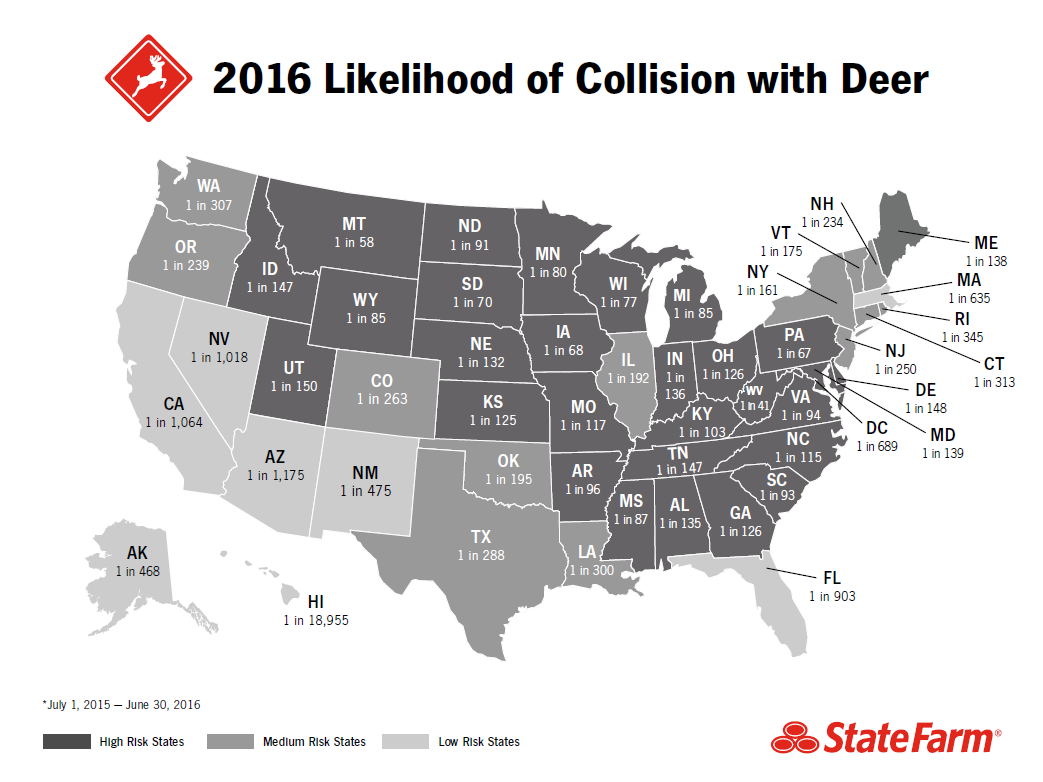
\includegraphics[scale=.23]{fig/Chicago_deer/1920_deermap.png}
	\label{deermap}
\end{figure}
\end{frame}

\begin{frame}{Overabundant Deer is a Problem: CWD}
\begin{figure}[ht]
\centering
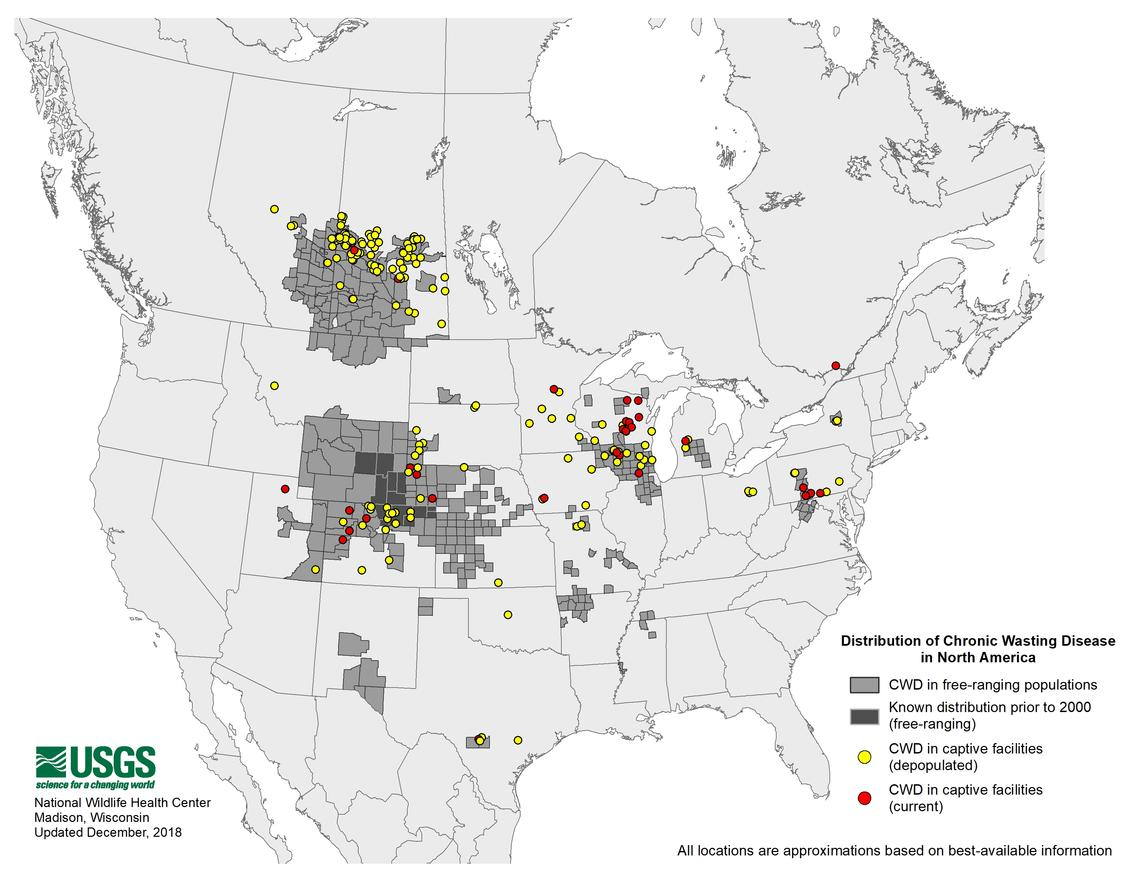
\includegraphics[scale=0.8]{fig/Chicago_deer/CWD.jpg}
\label{cwd}
\end{figure}
\end{frame}

\subsection{New Management Paradigm}

\begin{frame}{Paradigm Shift of Population Control}
\renewcommand\baselinestretch{1.5}\selectfont
	\begin{tabular}{r l l}
		\toprule
		Paradigms  &\textbf{Sustainable Harvest} &\textbf{Low Densities} \\ 
		\midrule
		\pause
	    Growth goal & $\sim1$  &$<1$ to reduce \\ \pause
	    Density & Various & Low \\ \pause
		Age structure & Stationary  & Non-stationary  \\
		\bottomrule
	\end{tabular}\pause
\renewcommand\baselinestretch{1}\selectfont
\\
\\
\\
\textbf{Requires a further evaluation!}
\end{frame}

\subsection{Research Objective}
\begin{frame}{Research Objective}
\renewcommand\baselinestretch{1.25}\selectfont
	\begin{itemize}
		\item Evaluate intensive harvest as a method of population control with a goal of maintain low density: \textbf{\\  Is intensive harvest effective?}\pause
		\item Understanding the dynamics of suburb deer population under such control: \textbf{\\  What is the best way to control it?}\pause
		\item Evaluate the effect of shifted age structure after intensive harvest: \textbf{\\  Can we skip a harvest year?}\pause
	\end{itemize}
\renewcommand\baselinestretch{1}\selectfont
\end{frame}

\section{Chicago Suburb Deer: a Case Study}
\begin{frame}
\LARGE{Chicago Suburb Deer: a Case Study}
\end{frame}

%\begin{frame}{Chicago Suburb Deer: a Case Study}
%	\begin{itemize}
%		\item Intensive harvest
%		\item Population Dynamics reconstruction
%		\item Test of age structure effect and culling schemes
%	\end{itemize}
%\end{frame}

\subsection{Intensive Harvest}
\begin{frame}{Study area: Complex 1}
\begin{columns}
	\begin{column}{0.3\textwidth}
		\begin{itemize}
			\item $30.6 km^2$ 
			\item Isolated by highways
		\end{itemize}
	\end{column}
	\begin{column}{0.7\textwidth}
		\begin{center}
			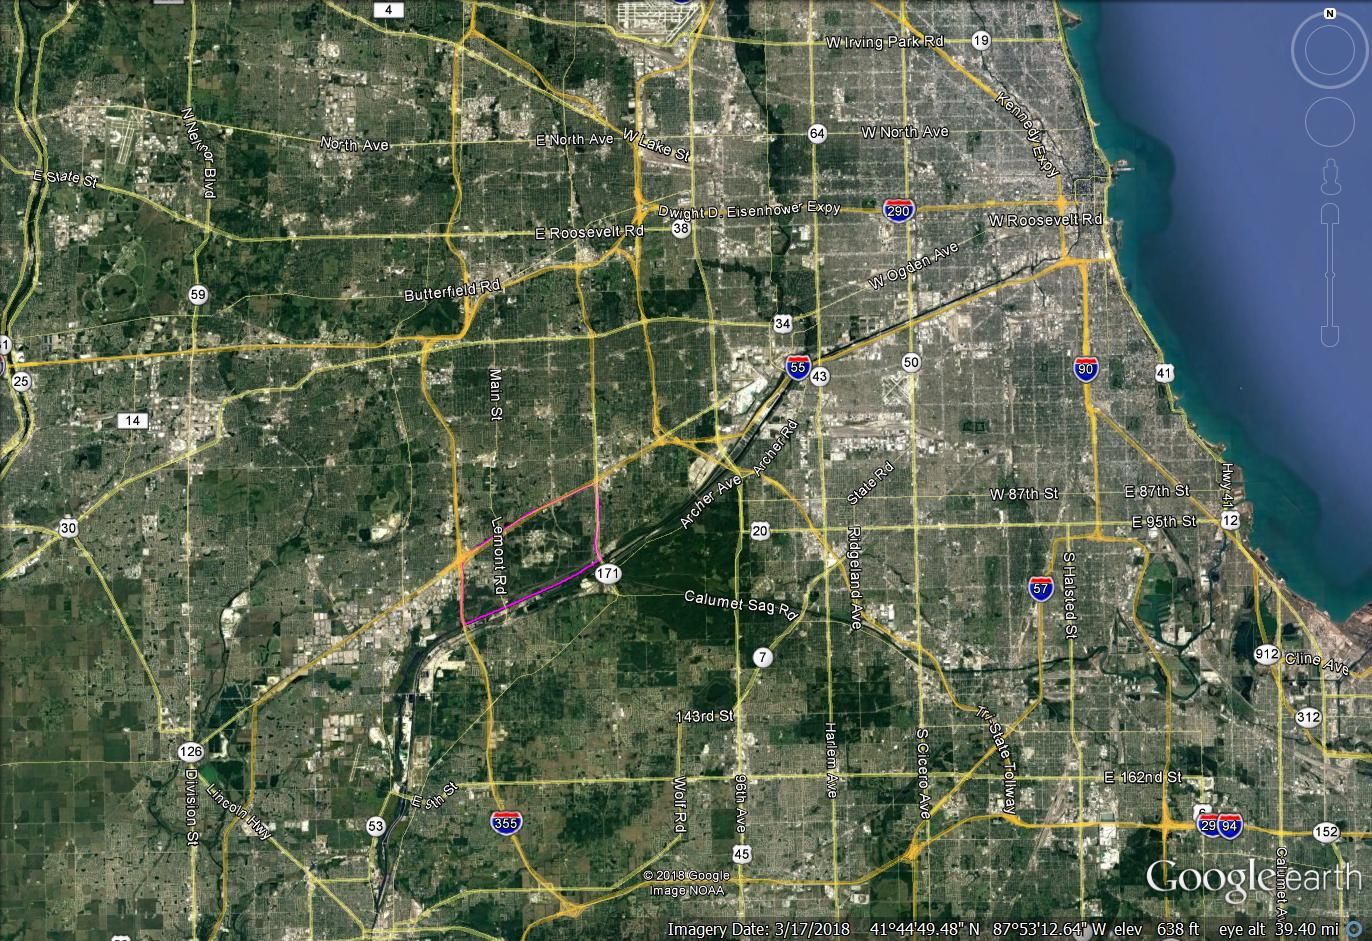
\includegraphics[width=\textwidth]{fig/Chicago_deer/Complex1.jpg} % should be map of complex 1  
		\end{center}
	\end{column}
\end{columns}
\end{frame}

\begin{frame}{Intensive harvest}
% put another column here for quick facts of number of harvested
\begin{columns}
	\begin{column}{0.3\textwidth}
		\begin{itemize}
			\item 15 years \pause
			\item 3,827 records
		\end{itemize}
	\end{column}
	\begin{column}{0.7\textwidth}
		\begin{center}
			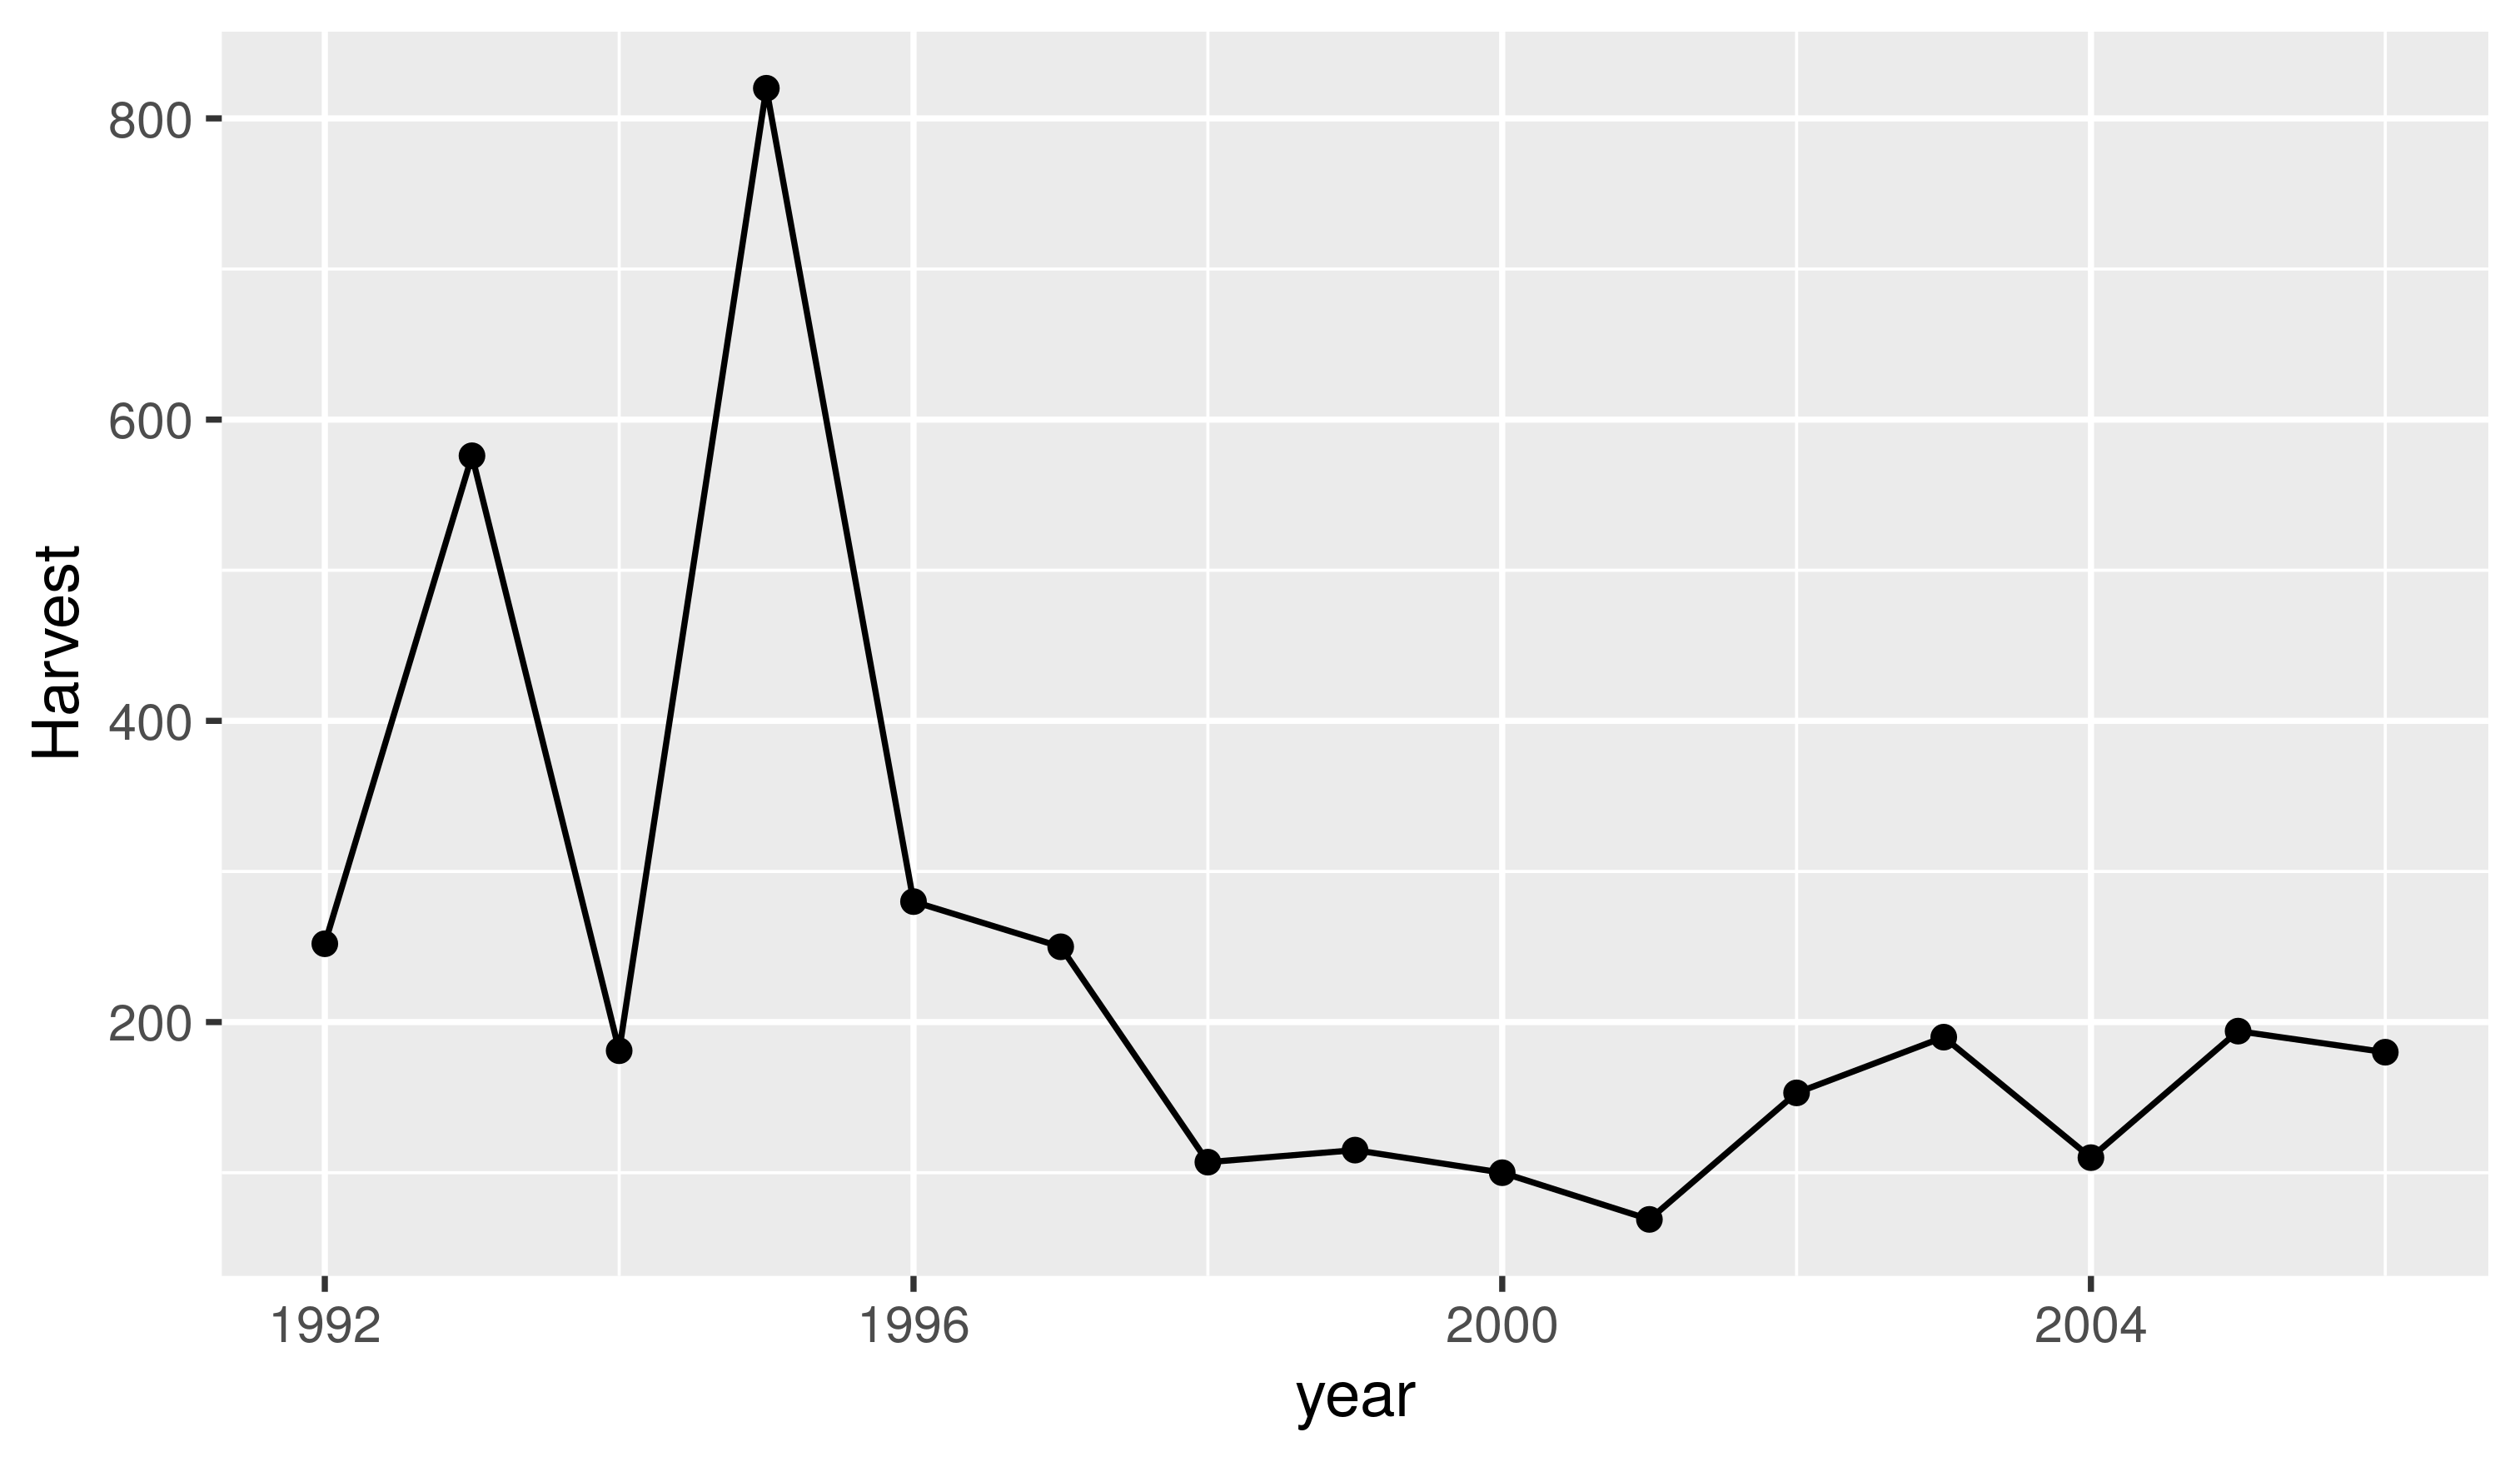
\includegraphics[width=\textwidth]{fig/Chicago_deer/totalharv.png}      
		\end{center}
	\end{column}
\end{columns}
\end{frame}

\begin{frame}{Questions to ask}
\renewcommand\baselinestretch{1.25}\selectfont
	\begin{itemize}
		
		\item Did this method work in Chicago? \pause
		\item What was the effect of shifted age structure after culling here? \pause
		\item Can we control by knock population down and then keep harvest a \textbf{fixed quota} or we have to be adaptive, i.e. try harvest a \textbf{fixed proportion}? \pause
		\item Which age should we focus on?\pause
	\end{itemize}
\renewcommand\baselinestretch{1}\selectfont
\end{frame}

\begin{frame}{To Answer These Questions:}
	Reconstruct the Dynamics and find the posterior distribution of population growth under different schemes!
\end{frame}

\subsection{Population Reconstruction: a Bayesian Approach}

\begin{frame}{Data Collected}
\renewcommand\baselinestretch{1.25}\selectfont
\begin{itemize}
	\item Age-at-harvest
	\item Post-harvest aerial count
	\item Fecundity was surveyed annually
	\item Prior knowledge from Etter et al. 2002 on survival rate
	
\end{itemize}
\renewcommand\baselinestretch{1}\selectfont
\end{frame}

\begin{frame}{Process Model: Leslie Matrix Projection}
\begin{figure}[ht]
	\centering
	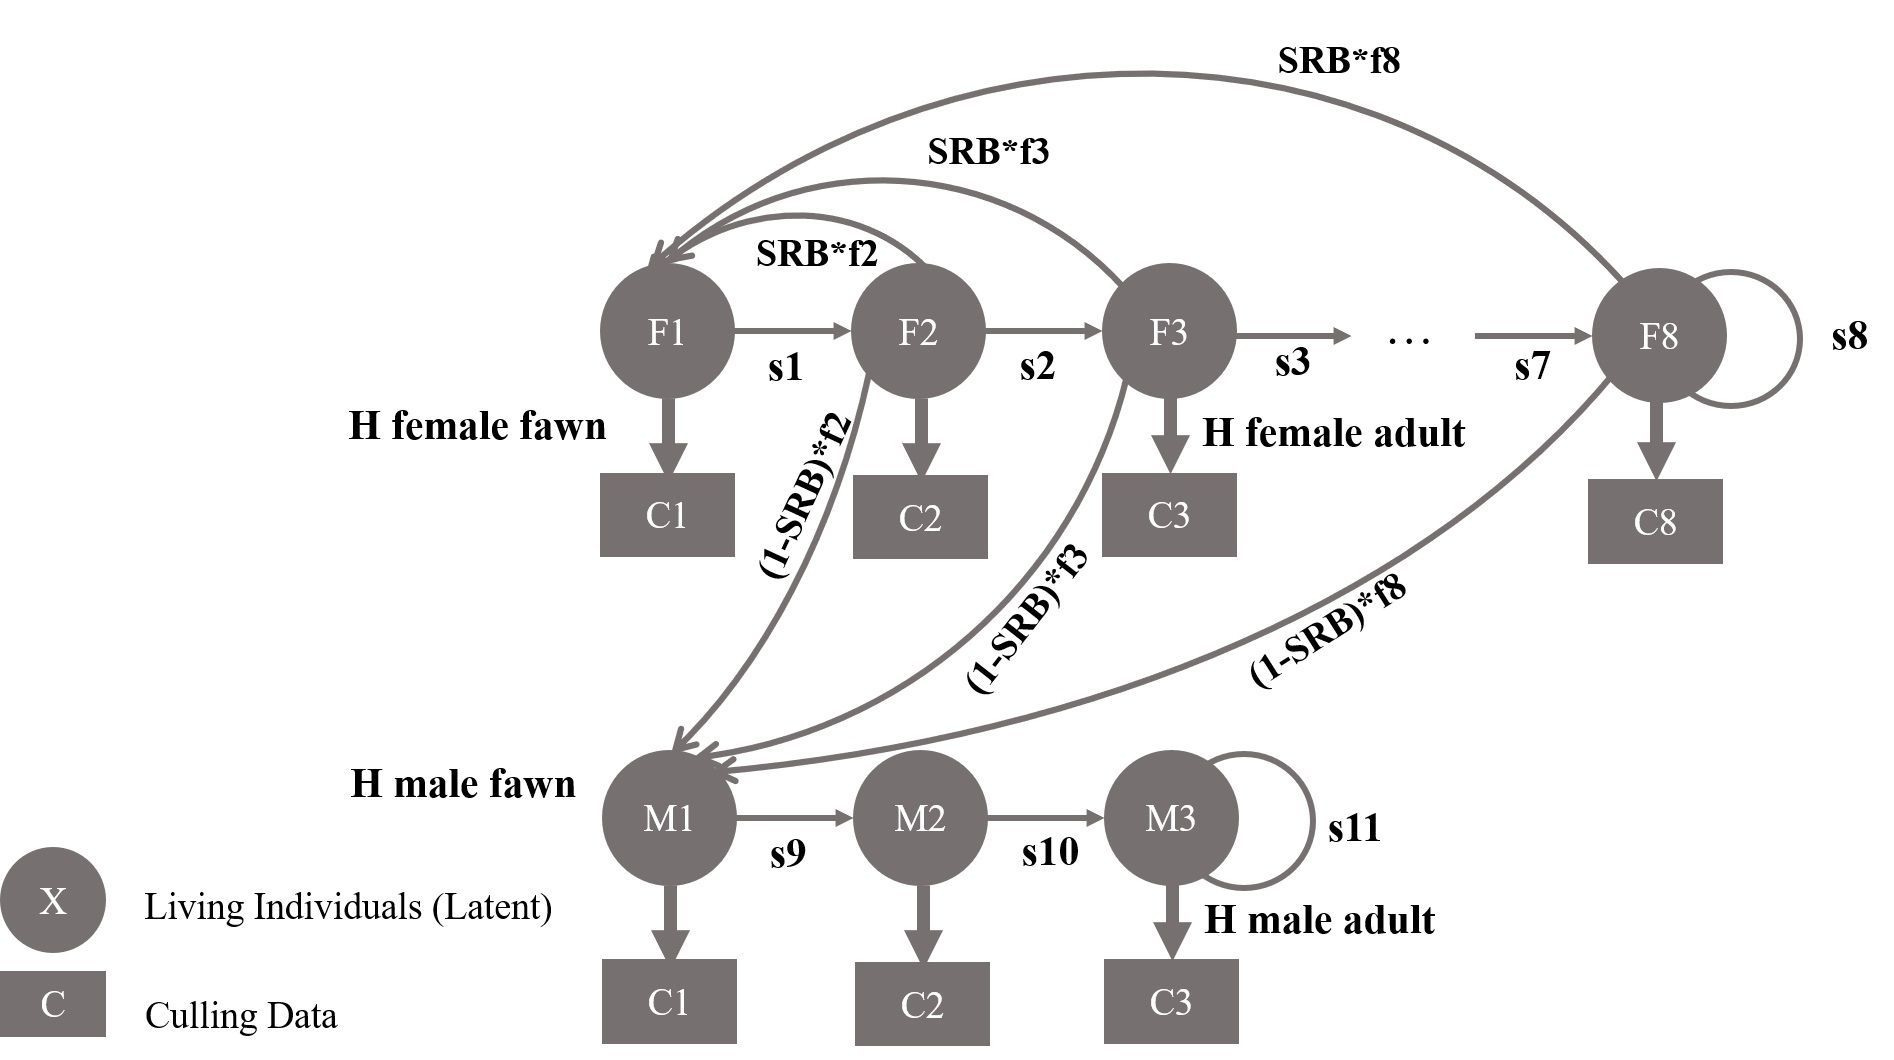
\includegraphics[width=\textwidth]{fig/Chicago_deer/LHD.jpg}
	\label{LHD}
\end{figure}
\end{frame}



\begin{frame}{Reconstruction: A Bayesian (Filter) Framework}
\begin{figure}[ht]
% you need to make a graph about the bayesian approach
	\centering
	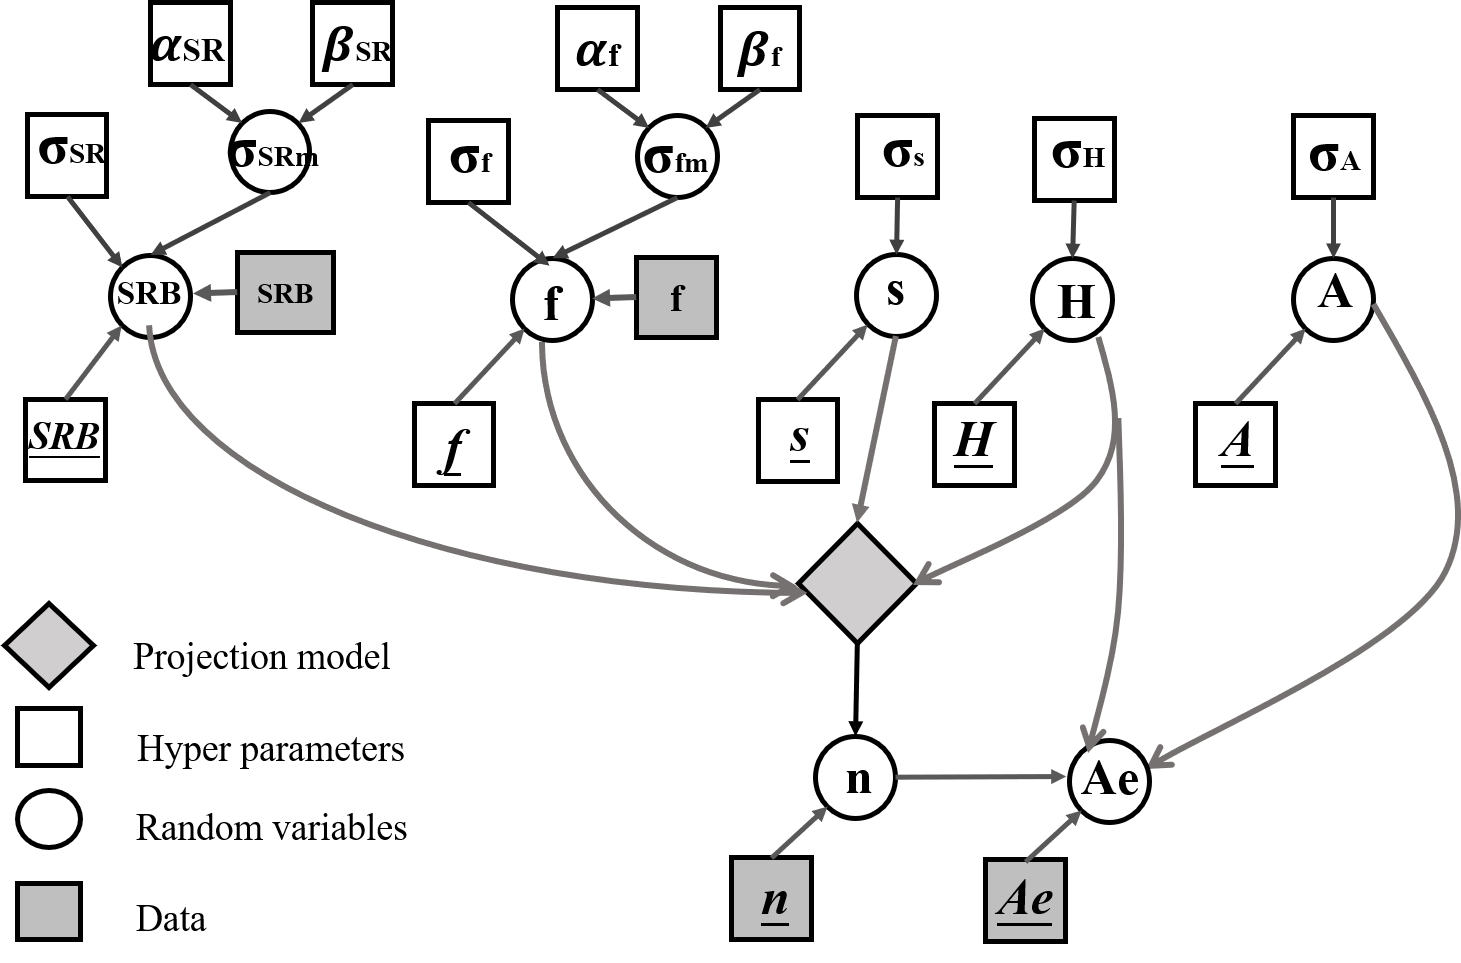
\includegraphics[width=0.8\textwidth]{fig/Chicago_deer/Bayes.png}
	\label{Bayes}
\end{figure}

{\footnotesize Algorithm Modified from Weldon et al. 2013 and implemented in R and C++}
\end{frame}

\begin{frame}{Model Selection Based on DIC}
\renewcommand\baselinestretch{1.25}\selectfont
\begin{itemize}
	\item There are multiple assumptions considered vital rates: e.g. whether fecundity changing through time and age?
	\item Model was selected based on \textbf{Deviation Information Criterion} (DIC), a Bayesian extension of AIC (Gelman et al. 2013).
\end{itemize}
\renewcommand\baselinestretch{1.25}\selectfont
\end{frame}

\begin{frame}{Making Predictions on Different Schemes}
\begin{itemize}
	\item Stochastic Leslie matrix model with vital rates follow posterior distribution estimated by reconstruction: a retrospect
	\item i.e., estimating the conditional distribution of population \textbf{given scheme and data}
	\[
	Population|Data,Scheme
	\]
\end{itemize}
\end{frame}

\subsection{Results}

\begin{frame}{Model Selection}
\renewcommand\baselinestretch{1.5}\selectfont
\begin{tabular}{ l l l l l  l}
	\toprule
	 Fecundity & Survival & Harvest & error  & $P_d$ & DIC \\ 
	\midrule
	 age, time  &  age, sex, time & F/A, sex, time & homo &224.6&1245\\ 
	 F/Y/A, time & age, sex, time & F/A, sex, time & time &205.0&1297 \\
	 F/Y/A, time & age, sex, time & F/A, sex, time & homo &206.3&1304 \\
	 F/Y/A, time & F/A, sex, time & F/A, sex, time & time &182.4&1307 \\
	\bottomrule
\end{tabular}\pause
\renewcommand\baselinestretch{1}\selectfont
\\
\\
\\
\textbf{Model 1 were chosen for predictions}
\end{frame}


\begin{frame}{Reconstructed Post-harvest Population}
We successfully control the population size to $\sim 300$
	\begin{figure}[ht]
		\centering
		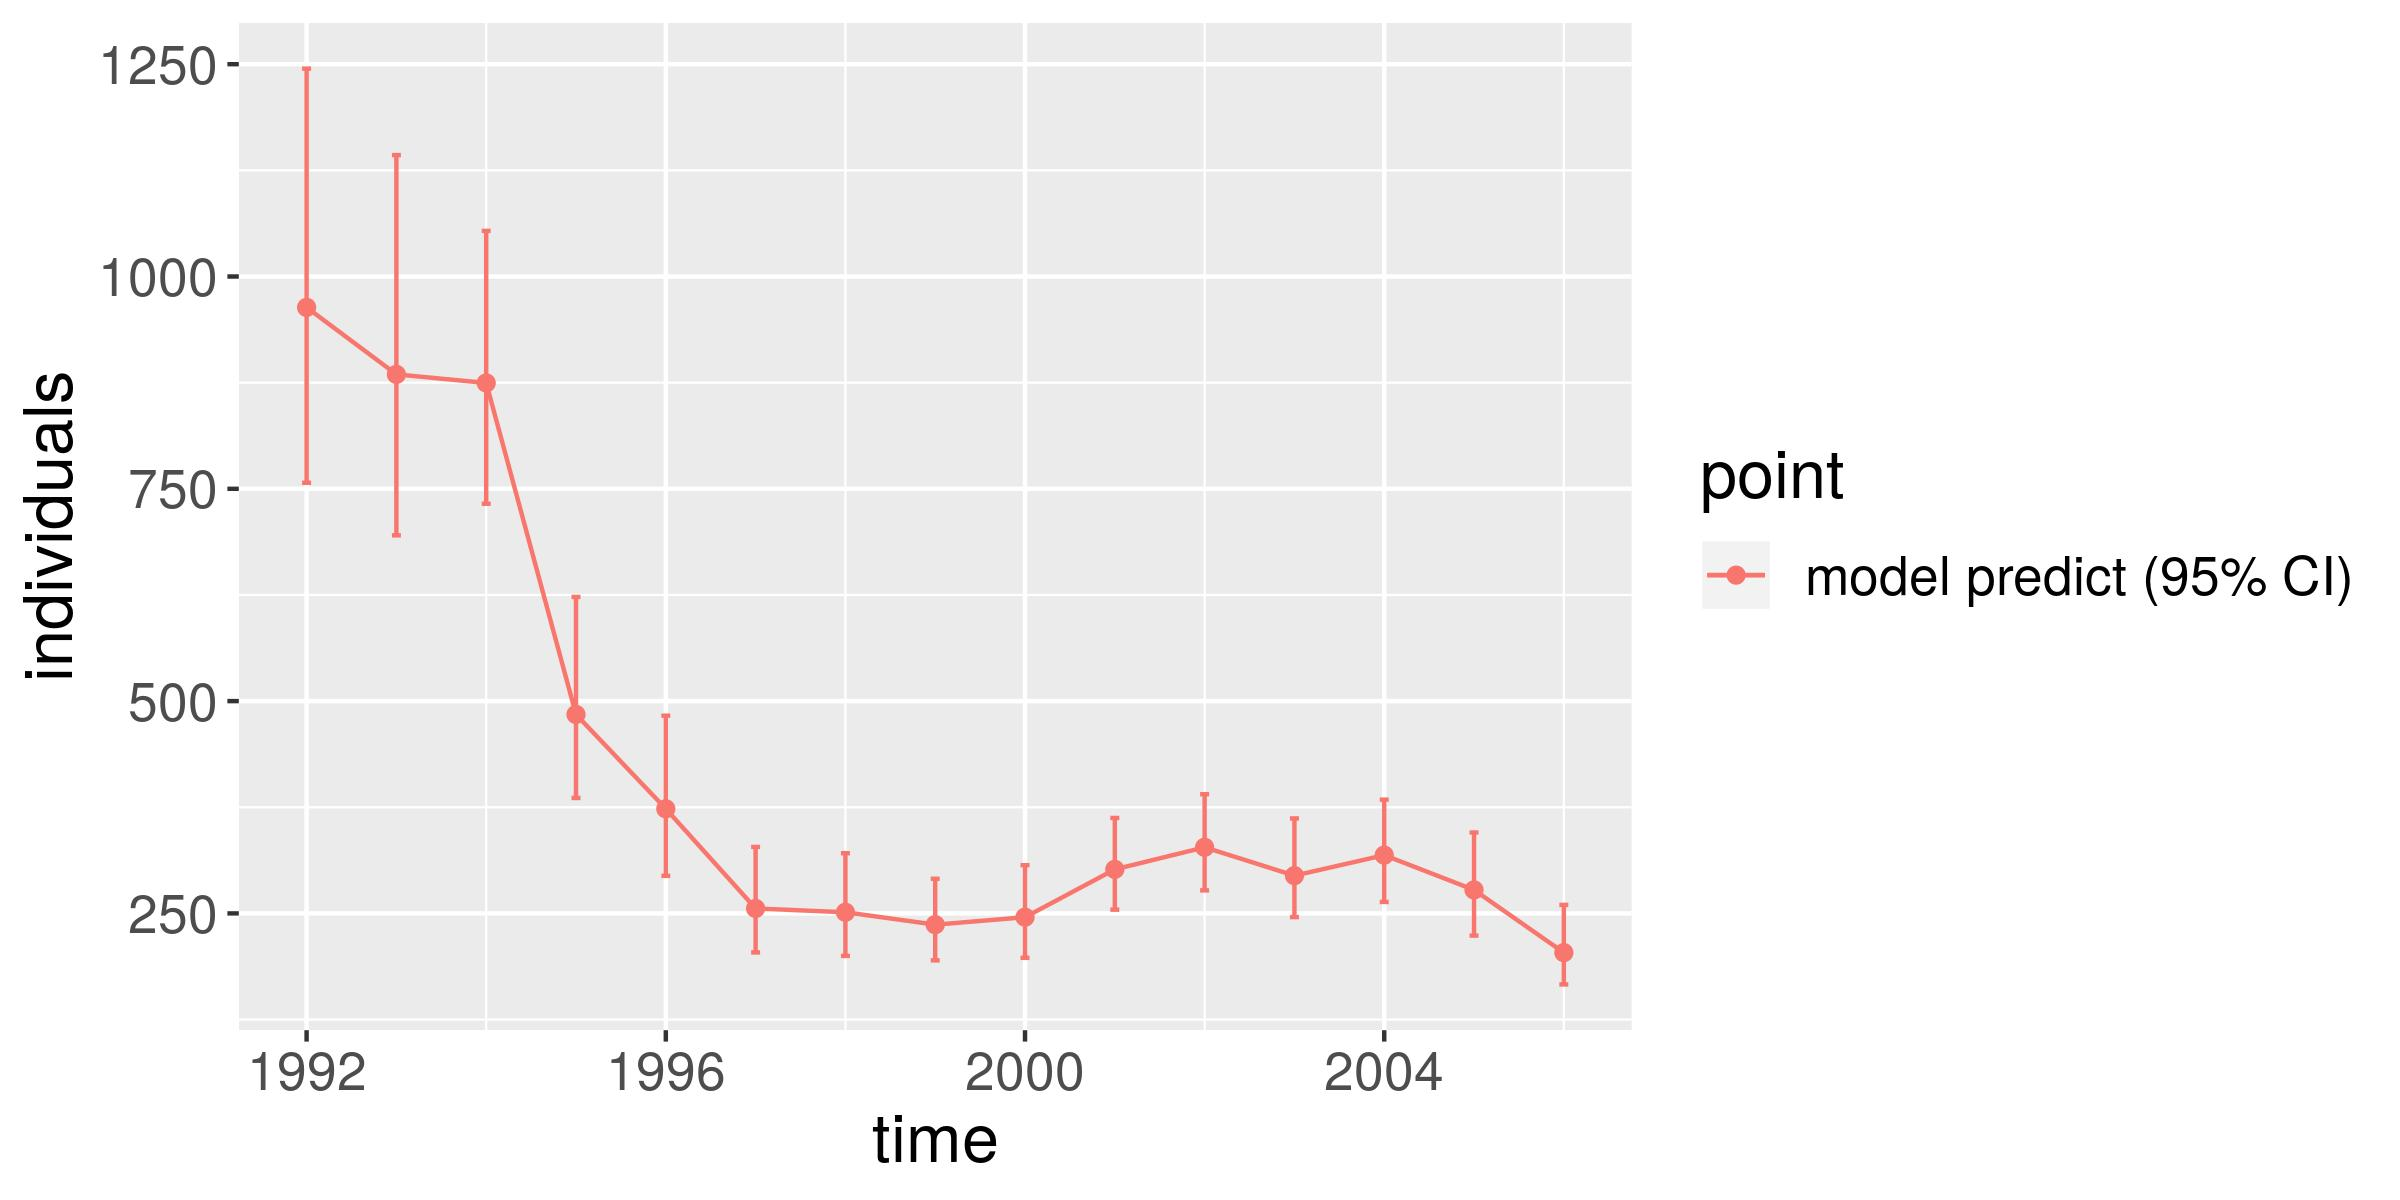
\includegraphics[width=\textwidth]{fig/Chicago_deer/post_harvest_popu.jpg}
		\label{postcull}
	\end{figure}
\end{frame}

\begin{frame}{Can Shifted Age Structure be an Insurance?}
In terms of growth rate: \textbf{No}
	\begin{figure}[ht]
		\centering
		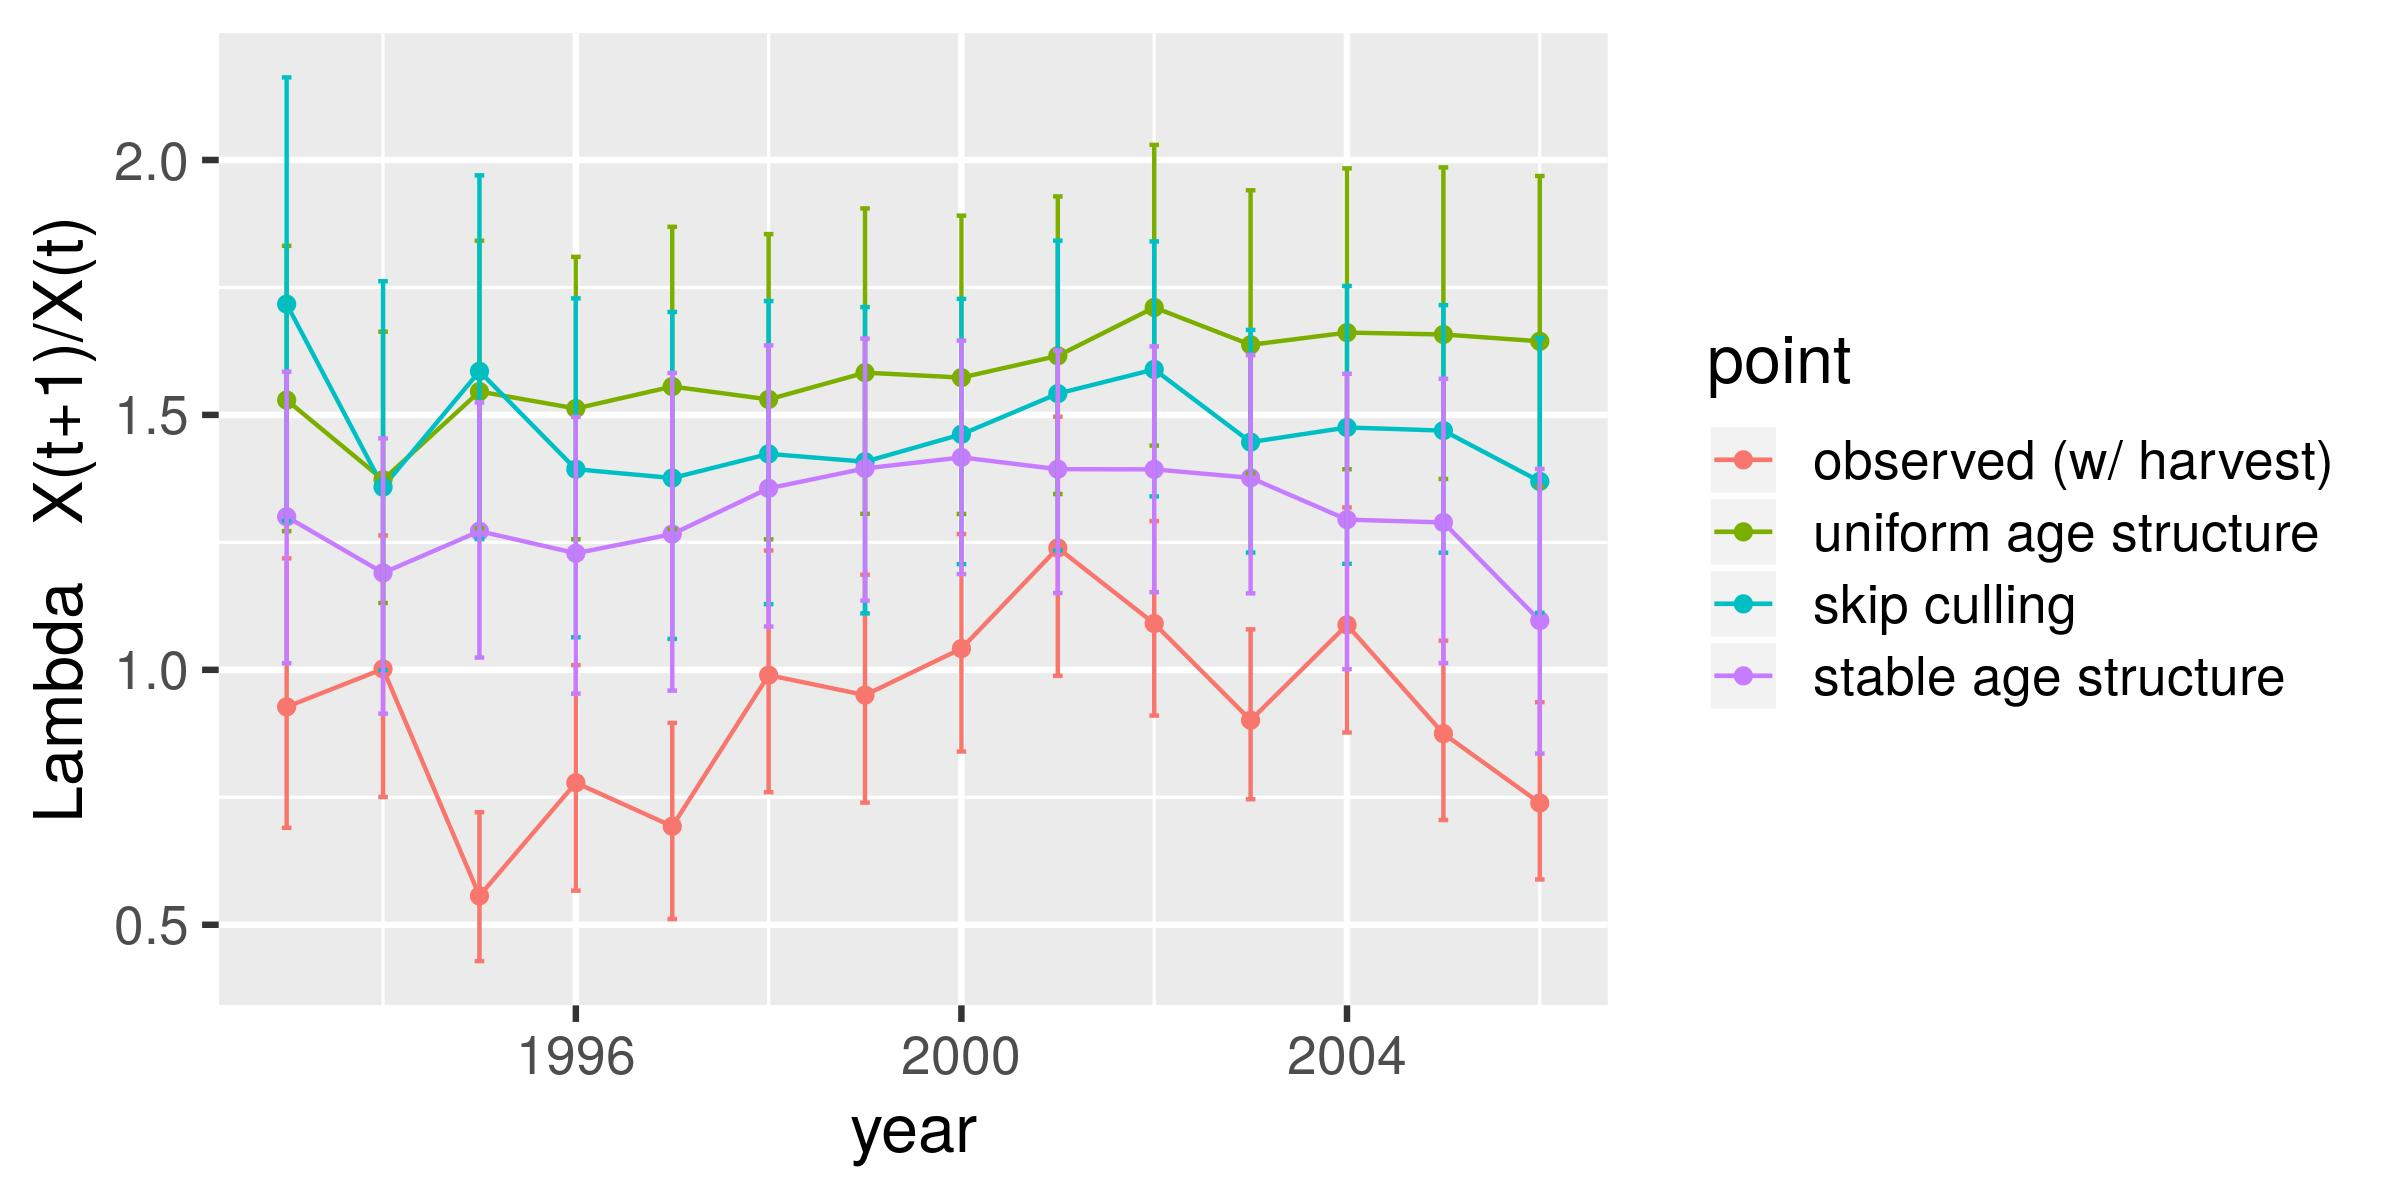
\includegraphics[width=\textwidth]{fig/Chicago_deer/Lambda.jpg}
		\label{lambda}
	\end{figure}
\end{frame}

\begin{frame}{Can Shifted Age Structure be an Insurance?}
But low population size itself can be one in terms of recruitment
\begin{figure}[ht]
	\centering
	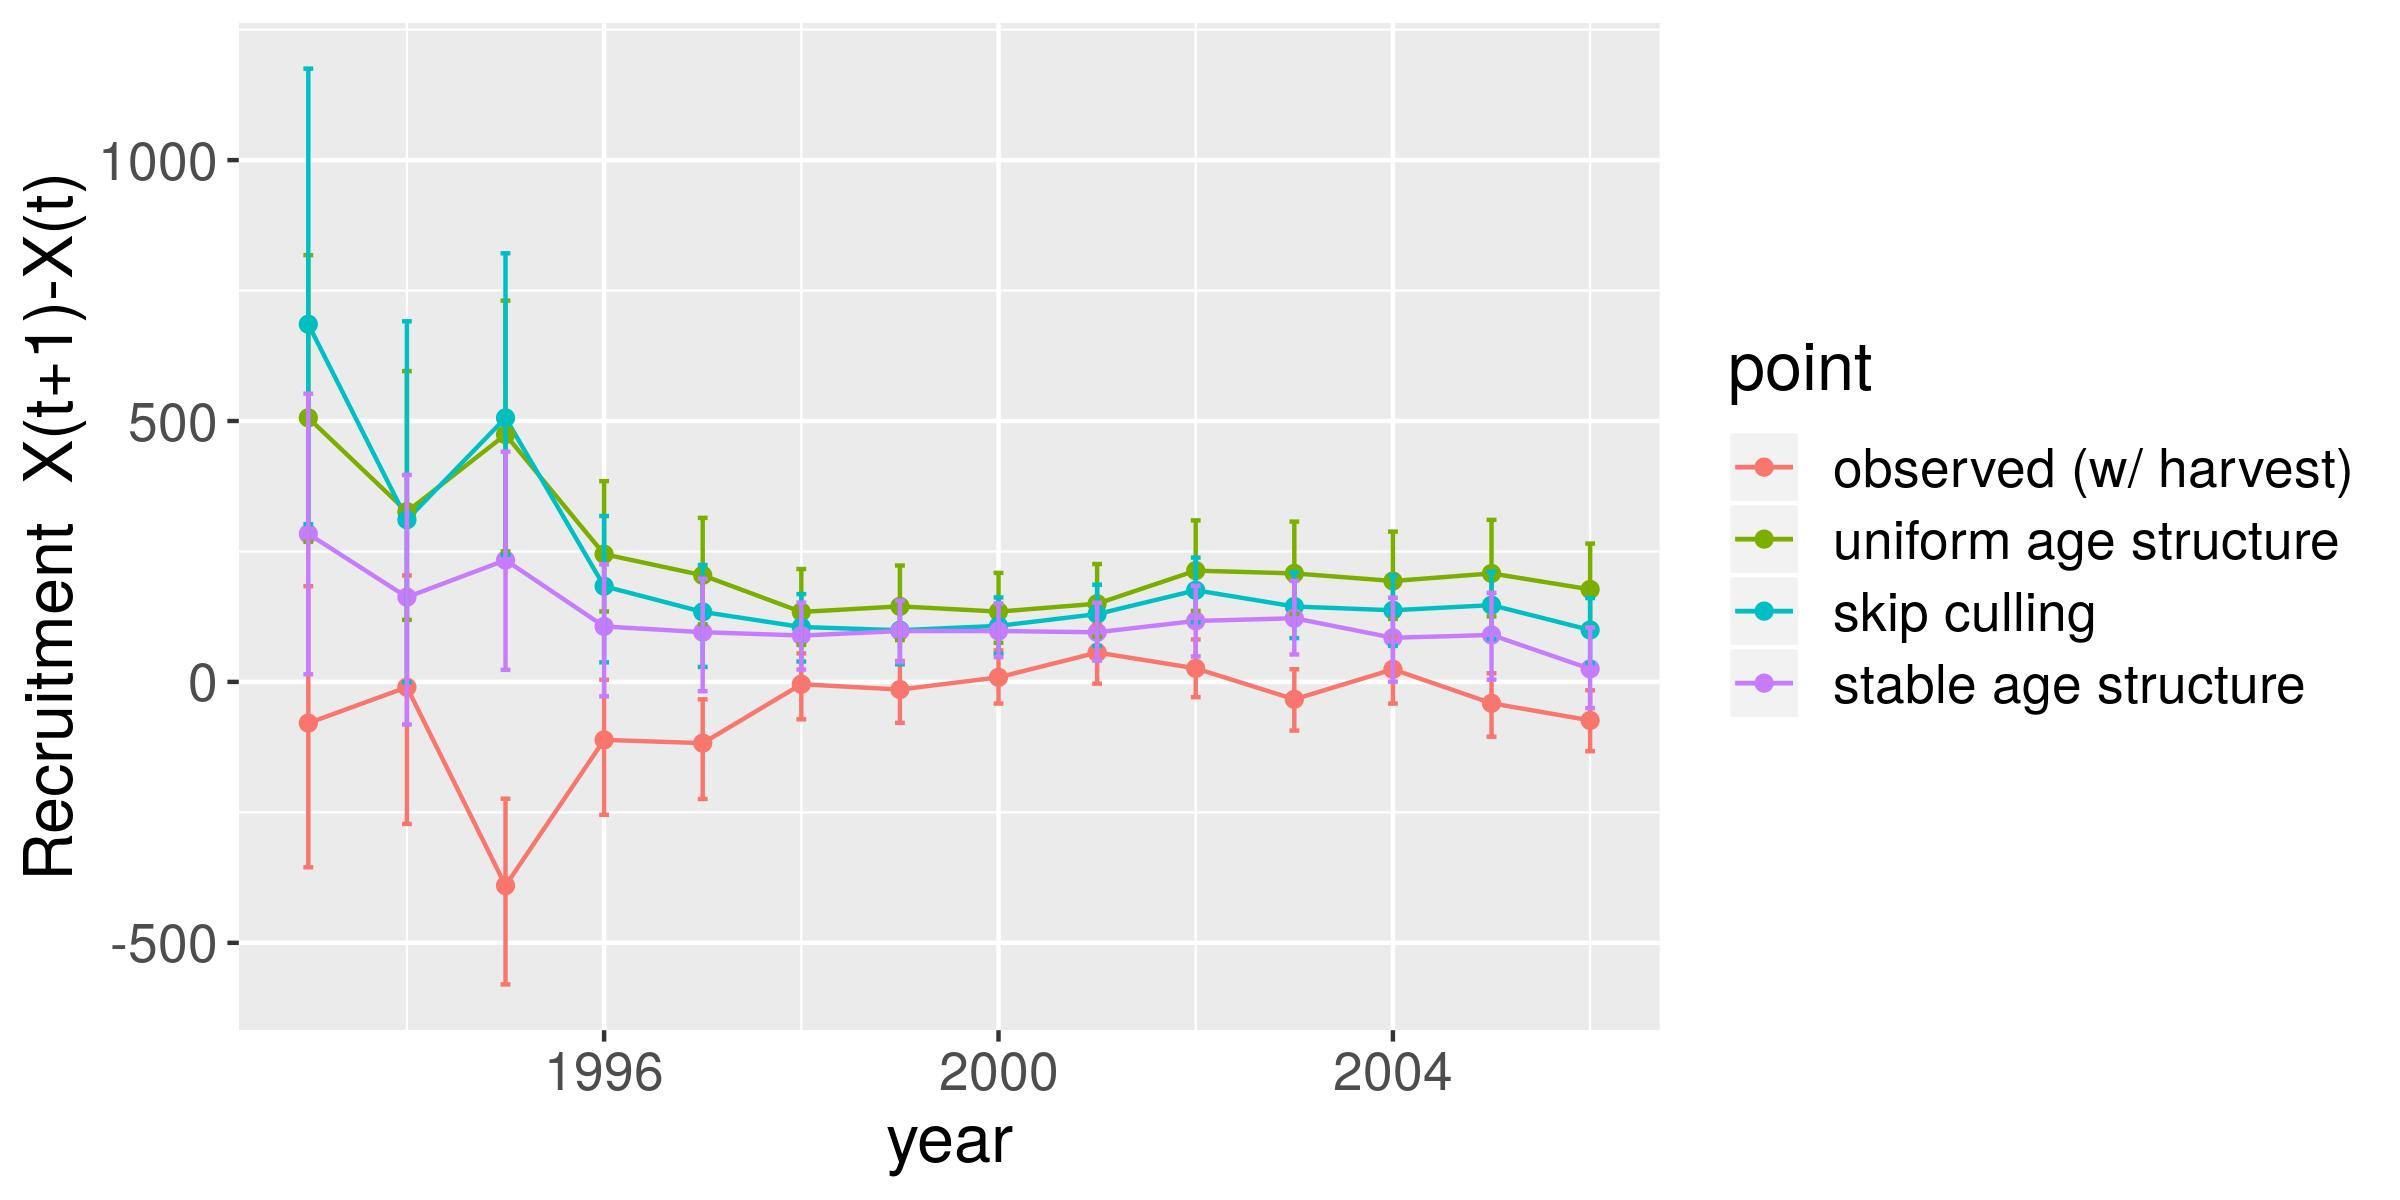
\includegraphics[width=\textwidth]{fig/Chicago_deer/Recu.jpg}
	\label{recru}
\end{figure}
\end{frame}

\begin{frame}{Culling amount: Fix quota vs Fix Proportion}
\begin{itemize}
	\item Retrospect: used quota/proportion and vital rates of  1992-2016\\
	\item Non-selective: Assuming we allocate the quota by age structure 
\end{itemize}
\end{frame}

\begin{frame}{Culling amount: Fix quota}
\begin{figure}[ht]
	\centering
	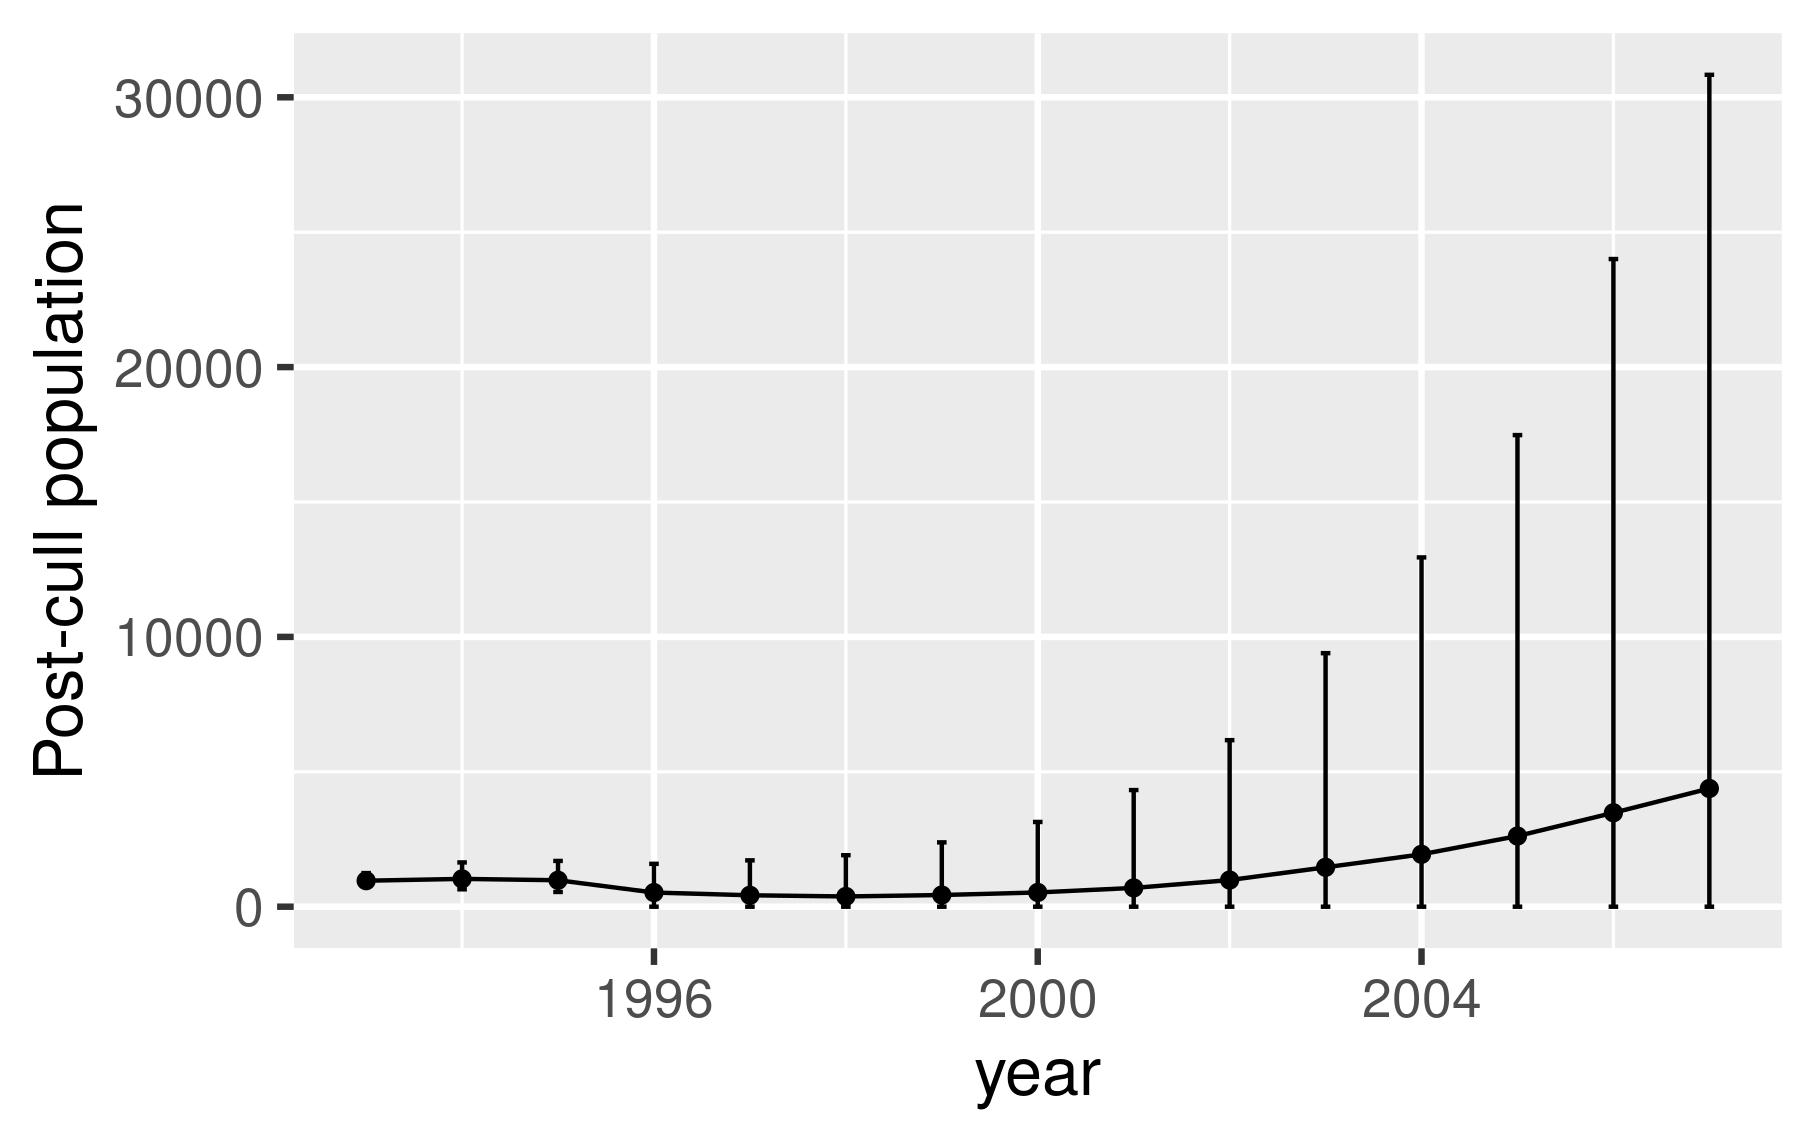
\includegraphics[width=0.8\textwidth]{fig/Chicago_deer/unif_quo.jpg}
	\label{quota}
\end{figure}
\end{frame}

\begin{frame}{Culling amount: Fix proportion}
\begin{figure}[ht]
	\centering
	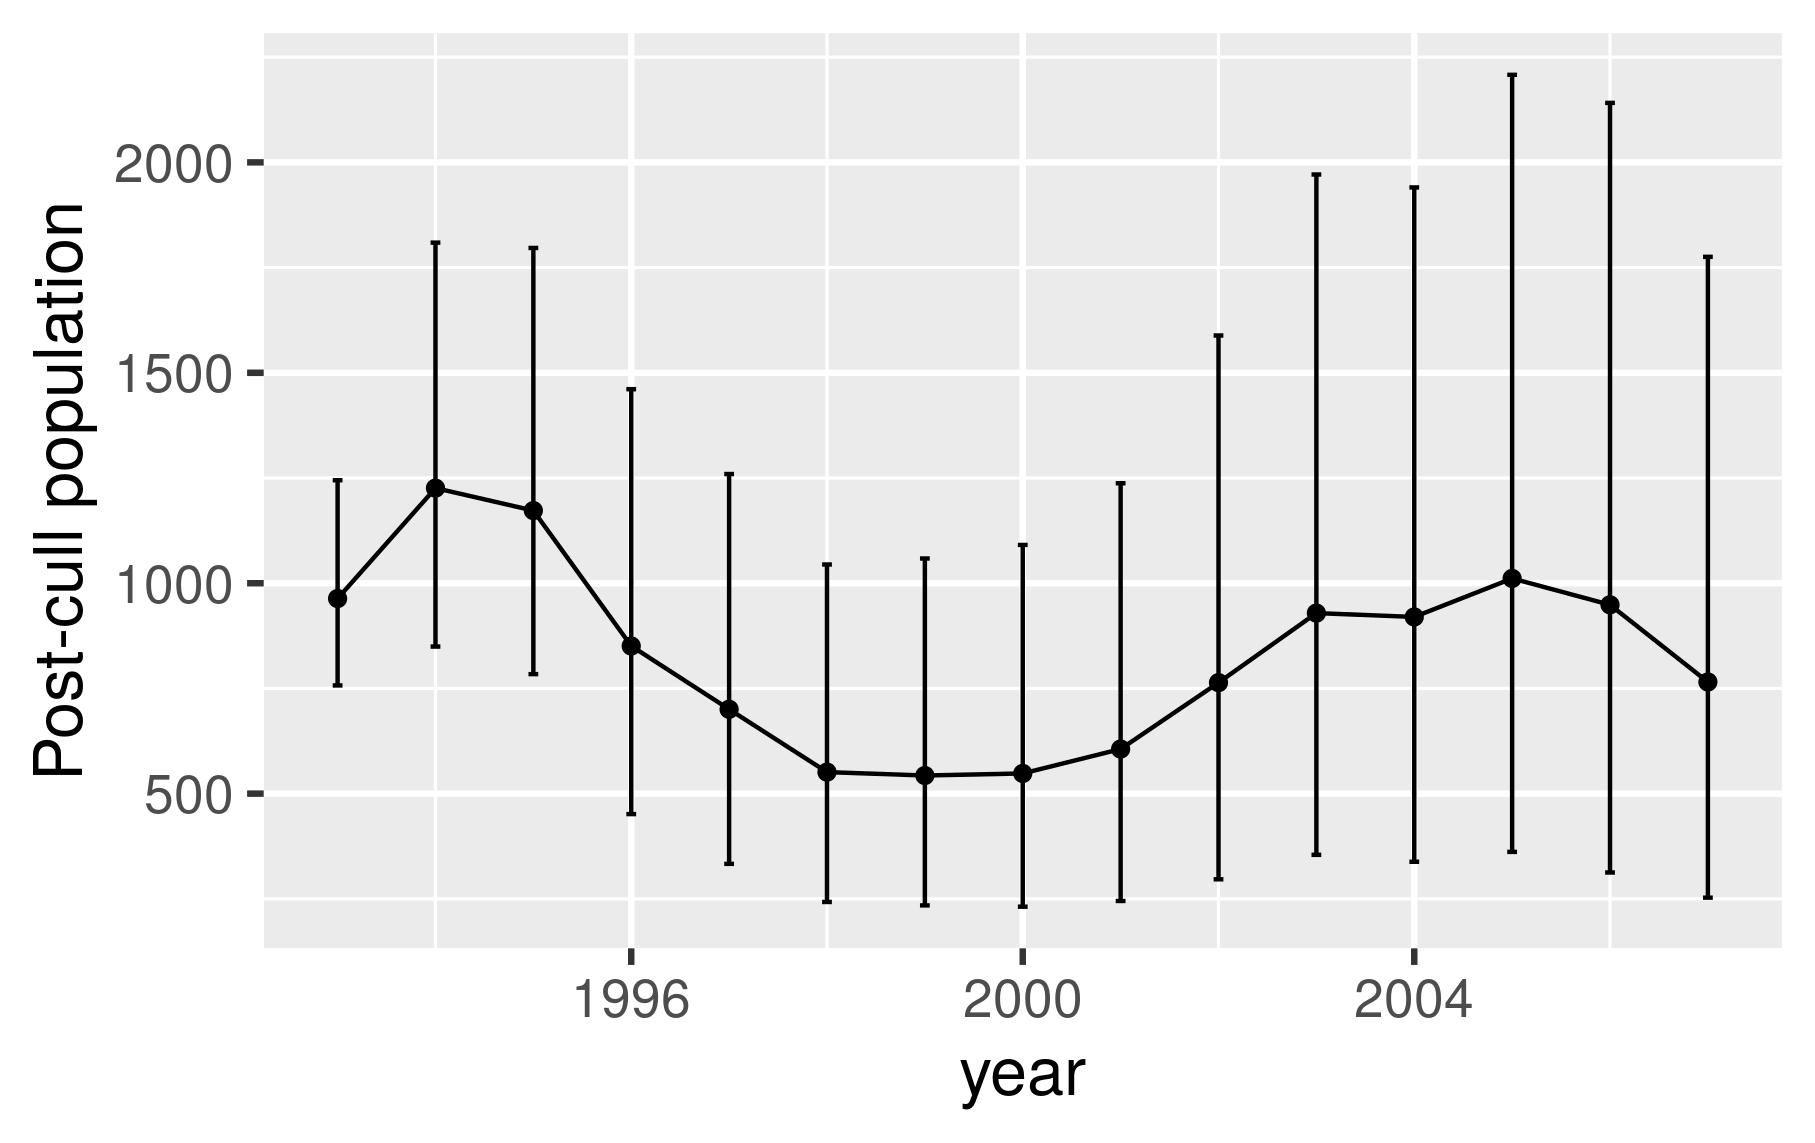
\includegraphics[width=0.8\textwidth]{fig/Chicago_deer/unif_por.jpg}
	\label{proportion_unif}
\end{figure}
\end{frame}

\begin{frame}{Selective Culling: Which age?}
\begin{itemize}
	\item Retrospect: used proportion and vital rates of  1992-2016\\
	\item Selective: added a weight to each age 
\end{itemize}
\end{frame}

\begin{frame}{Selective Culling: Doe twice likely to be harvested}
\begin{figure}[ht]
	\centering
	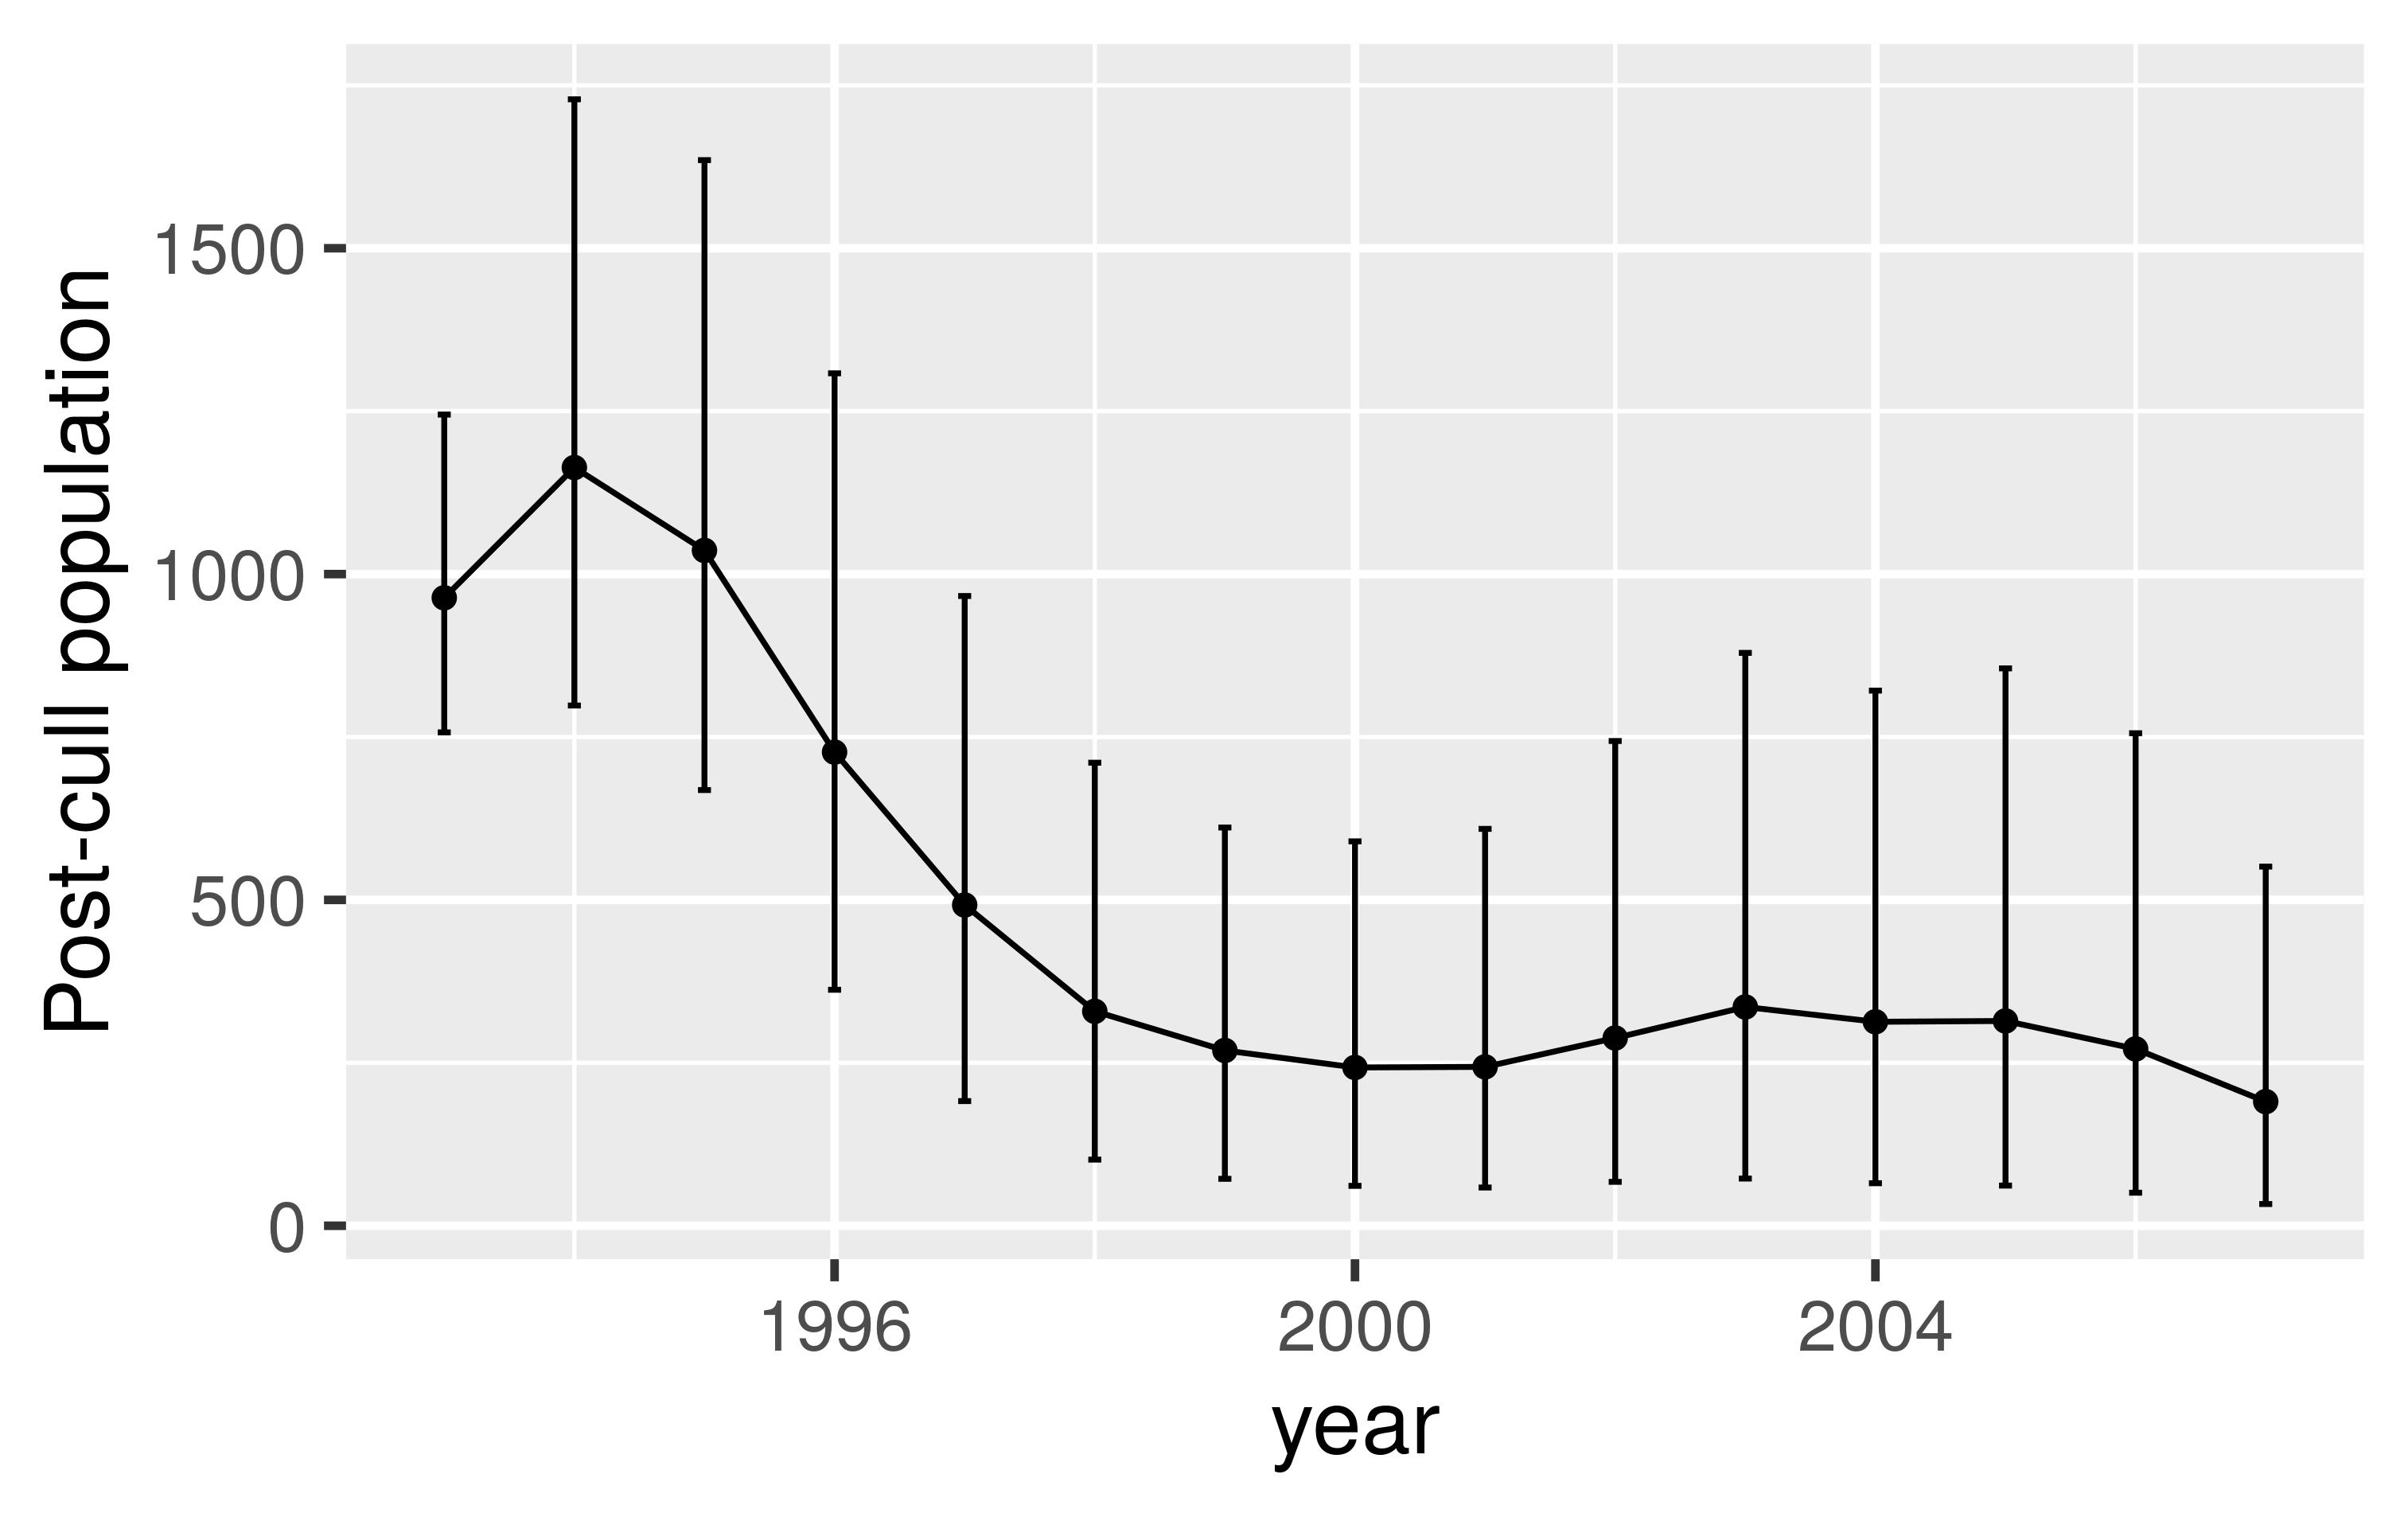
\includegraphics[width=0.8\textwidth]{fig/Chicago_deer/more_doe_porprotion.jpg}
	\label{proportion_moredoe}
\end{figure}
\end{frame}

\begin{frame}{Selective Culling: Only doe}
\begin{figure}[ht]
	\centering
	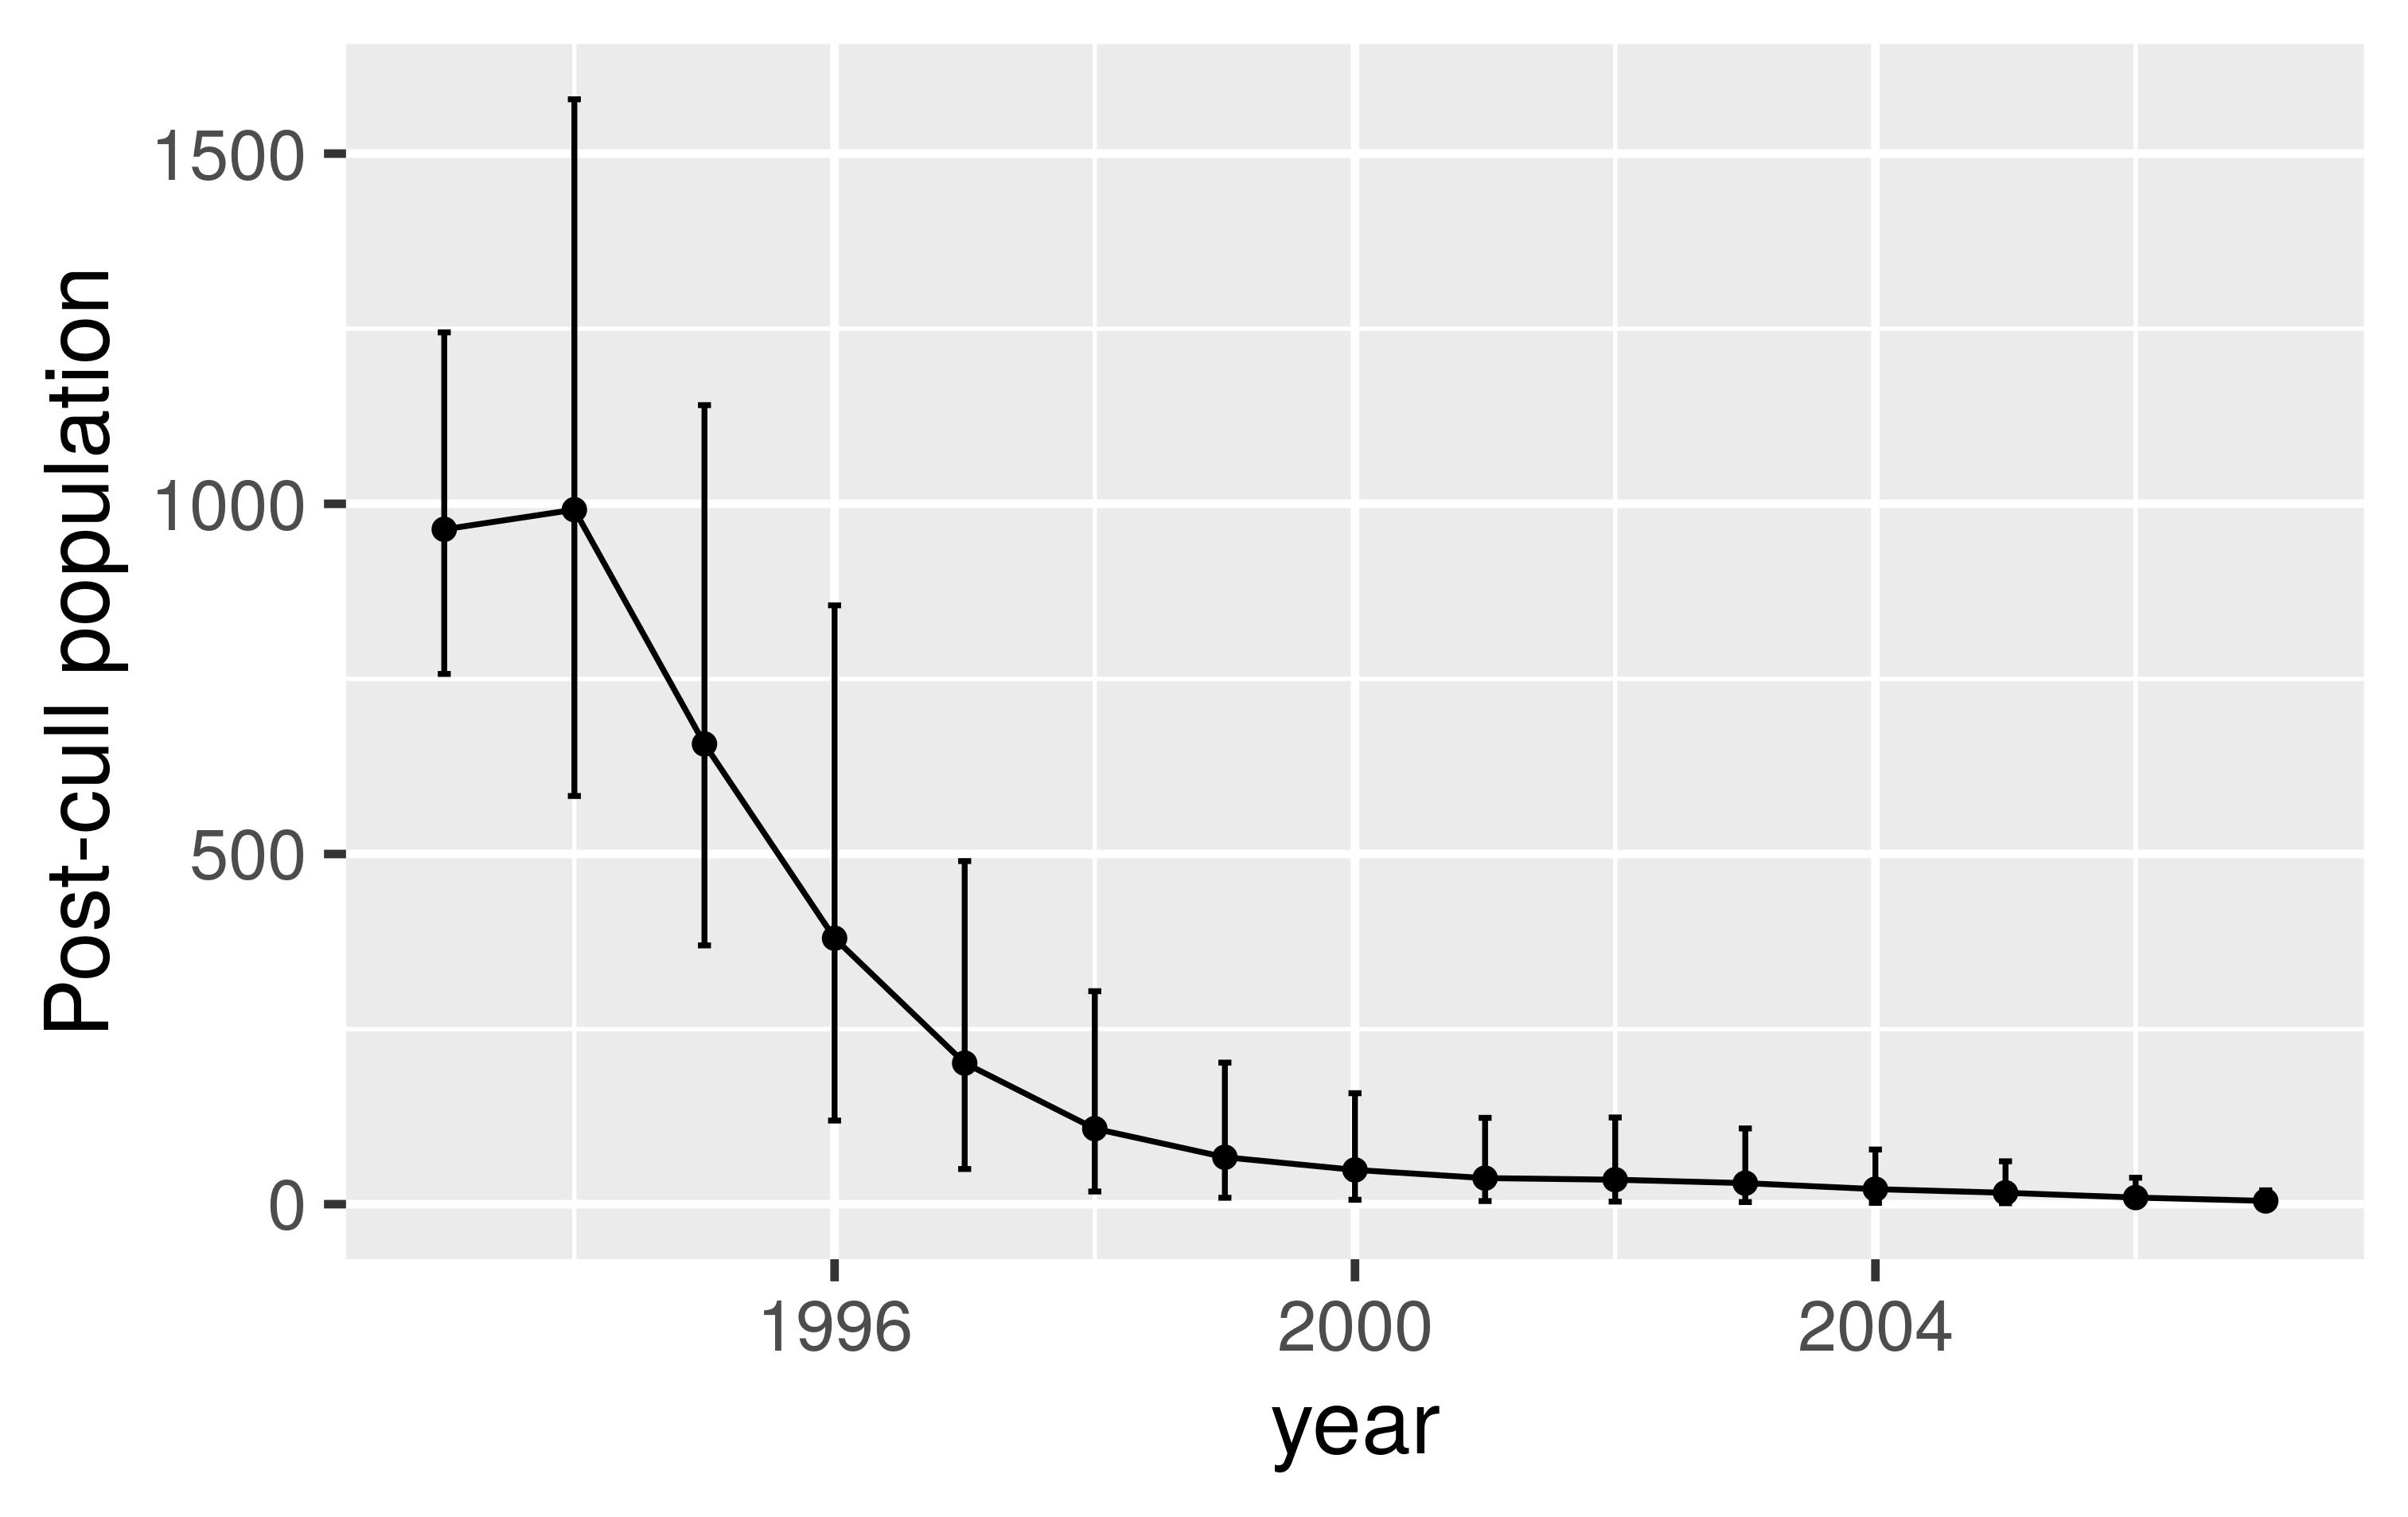
\includegraphics[width=0.8\textwidth]{fig/Chicago_deer/only_doe.jpg}
	\label{proportion_onlydoe}
\end{figure}
\end{frame}

\begin{frame}{Selective Culling: Only doe, fix quota}
\begin{figure}[ht]
	\centering
	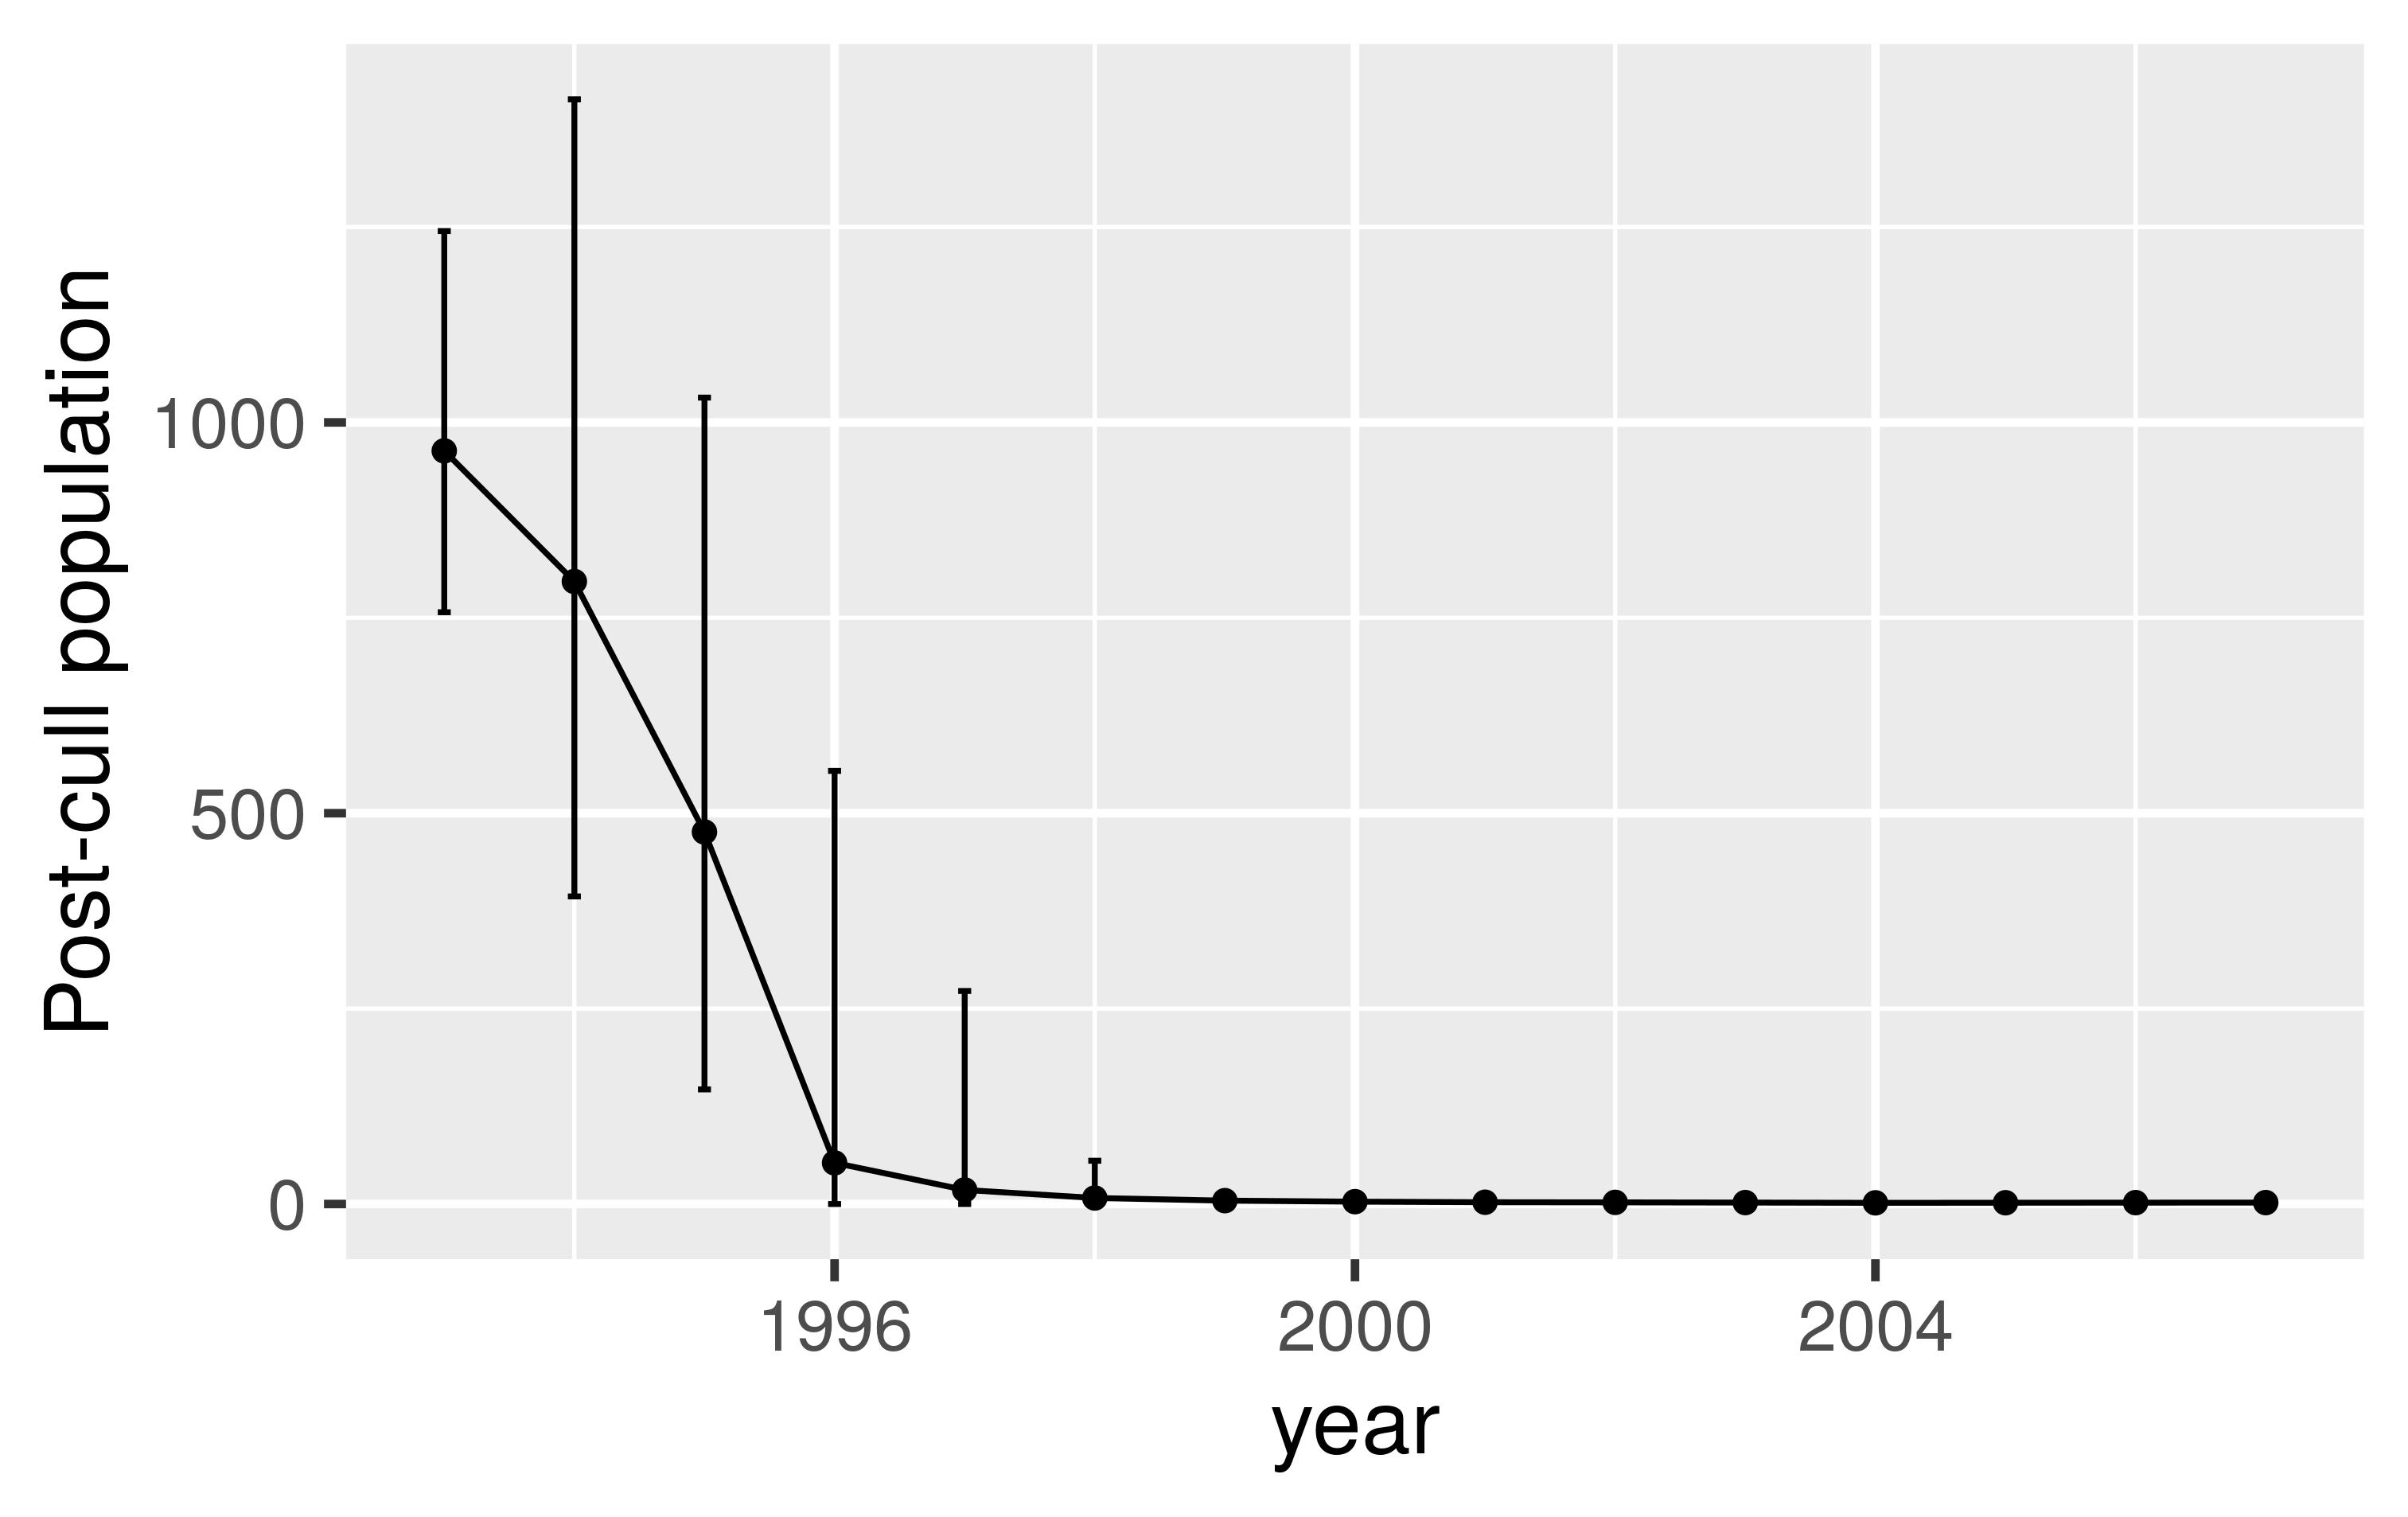
\includegraphics[width=0.8\textwidth]{fig/Chicago_deer/only_doe_quota.jpg}
	\label{quota_onlydoe}
\end{figure}
\end{frame}

\begin{frame}{Take Home Message for Management Based on This Case}
\begin{itemize}
	\item Intensive culling is a powerful tool for controlling overabundant deer \pause
	\item Continuous effort should be put in to control the population \pause
	\item After knocking the population down, the (adaptive) \textbf{fixed proportion} rather than fix quota harvest can help keeping the population low (this may means \textbf{similar effort} each year) \pause
	\item Be selective and focus on doe
\end{itemize}
\end{frame}

\section{References and others}

\begin{frame}{References}
	\begin{itemize}
		\item Etter, D. R., Hollis, K. M., Van Deelen, T. R., Ludwig, D. R., Chelsvig, J. E., Anchor, C. L., and Warner, R. E. (2002). Survival and movements of white-tailed deer in suburban chicago, illinois. The Journal of Wildlife Management, pages 500–510.
		\item Wheldon, M. C., Raftery, A. E., Clark, S. J., and Gerland, P. (2013). Reconstructing past populations with uncertainty from fragmentary data. Journal of the American Statistical Association, 108(501):96–110.
		\item Gelman, A., Carlin, J. B., Stern, H. S., Dunson, D. B., Vehtari, A., and Rubin, D. B. (2013). Bayesian data analysis. Chapman and Hall/CRC.
	\end{itemize}
\end{frame}


\begin{frame}{Acknowledgments}
\begin{itemize}
	\item Thank Michigan DNR officers who collected these data when I was not born
	\item Thanks my lab mates for all the discussions 
	\item Special thank to Department of Chemistry, UW-Madison for offering me TAship to fund my study in UW-Madison
\end{itemize}
\end{frame}

%\begin{frame}{An ad}
%	I am looking for PhD positions starting fall 2021, send me an email at \textbf{yshen99@wisc.edu} if you or someone you know are interested in!
%\end{frame}

\begin{frame}
	\LARGE{Questions?}
	\\
	\\
	\\
	{\footnotesize Open source statement: \\
	 All source code (in R and C++) can be find on Github repo YunyiShen/ReCAP, source code of this report can be found in repo  YunyiShen/UW-Course-Projects under GPL 3.0}
\end{frame}

\begin{frame}{Optimal/Worst Age Structure of Annual Growth}
	Consider a Leslie matrix $A$ and a population $X$, the growth rate can be written as:
	\[
	\begin{aligned}
	\lambda&=\frac{1^TAX}{1^TX}\\
	&=(1^TA)\frac{X}{1^TX}
	\end{aligned}
	\]
	This equals to the \textbf{weighted average} of $1^TA$, which is the column sum of Leslie matrix $A$, and we have
	\[
	min(1^TA) \le \lambda \le max(1^TA)
	\]
	
	will take equal when all individuals are at the age that maximize/minimize column sum of Leslie matrix, so: healthy fat doe/naive male fawn
\end{frame}


\end{document}
